\input{../../../Skript_praeambel.tex}
\addbibresource{BibliographyGRL.bib}

% !TeX spellcheck = en_US 

\begin{document}
%Ben�tigte Angaben f�r die Titelseite
\title{Summary of the lecture \\ \glqq MA INF 4316 - Graph Representation Learning\grqq\! \\ by Dr. Pascal Welke \\ (WiSe 2021/2022)}
%Hier Zeilenumbruch durch \\, da \newline in dieser Umgebung nicht funktioniert.
\author{Fabrice Beaumont \\ Matrikel-Nr: 2747609 \\
Rheinische Friedrich-Wilhelms-Universit�t Bonn}

%Erstellung des Titels
\maketitle
\tableofcontents
%\listoffigures

%----------------------------------------------------------

% Lec6 - p.44/52 - Left over \subset in the first line
% Lec7 - p. ...

%%%%%%%%%%%%%%%%%%%%%%%%%%%%%%%%%%
%%%%% Lecture 00 - 11.10.2021 %%%%
%%%%%%%%%%%%%%%%%%%%%%%%%%%%%%%%%%
%TODO: ANKI bis hier
\setcounter{chapter}{-1}
\chapter{Motivations - Learning Tasks on Graphs}
In this chapter we discuss different learning tasks on graph structured data.

A graph is a type of data structure which describes relationships (edges) between objects (vertices). For more formal definitions see  definitions \ref{def:UndirectedGraph} and \ref{def:DirectedGraph}. Family trees, social network connections and molecules are examples for graphs.

Graphs may incorporate much information in form of attributes. Vertices for example may correspond to persons and may be attributed by name, age or gender. In this example edges may additionally contain information about relationship properties. Another example are molecular graphs, which have atom types as vertex labels and their edges indicate the type of covalent bond.

The three main learning paradigms of machine learning are:
\begin{itemize}
	\item \textbf{Supervised Learning}: Find a data-consistent function that maps input to output values. In other words, given a set of training data $X=\{(x,f(x))\}$, find a hypothesis function $h\in\mathcal{H}$ such that $h\approx f$.\\
	(E.g. Linear Regression, Logistic Regression, Support Vector Machines, Nearest Neighbor, Naive Bayes Classifier, Decision Trees \& Random Forests, (Deep) Neural Networks, \dots)
	\item \textbf{Unsupervised Learning}: Find structures by identifying data correlations without explicit knowledge of memberships.\\
	(E.g. clustering, auto-encoders, (frequent) pattern mining, \dots)
	\item \textbf{Reinforcement Learning}: Learn a function which maximizes the cumulative output rewards by choosing appropriate actions in an unknown environment.\\
	(Search space exploration to reason about the environment.)	
\end{itemize}

Common supervised learning tasks on graphs are:
\begin{itemize}
	\item Assign a color to unknown vertices
	\item Predict likely new edges
	\item Predict unknown graph class
\end{itemize}

Common unsupervised learning tasks on graphs are:
\begin{itemize}
	\item Vertex clustering, Community detection
	\item Graph clustering
	\item Link prediction without supervision
\end{itemize}

The central problem of learning on graphs is how traditional machine learning approaches can be applied to graphs.

Linear Regression, Logistic Regression, Naive Bayes Classifiers, Decision trees and Random Forests expect \textit{tabular data}, i.e. a set of example with a known, fixed set of features.

One may consider to use features of vertices to learn on them. But several non-trivial questions arise, for example:\begin{itemize}
	\item How to deal with connections between vertices?
	\item How to deal with vertices without features?
	\item What if the objects we want to learn from are graphs themselves? (Possibly with different numbers of vertices or edges.)
\end{itemize}

Note that the usage of a graph's adjacency matrix as vector representation is not desirable, since isomorphic graphs can be represented in different adjacency matrices.

Another approach to make traditional machine learning approaches applicable to graphs is to use \textbf{graph representations}. These vectorize data with respect to task specific properties. Generally, we seek approaches that incorporate aspects of the graph's structure.

It is highly non-trivial to determine which information crucial for a specific learning task shall be represented in which way in the graph representation.

\paragraph{Example - Vertex classification:} Consider the graph depicted in Figure \ref{fig:vertexclassificationexample} and the task to reason about the color of unknown vertices by looking at training data.

\begin{figure}[H] %TODO: Is this image TeXed? Lecture 0 Slide 30
	\centering
	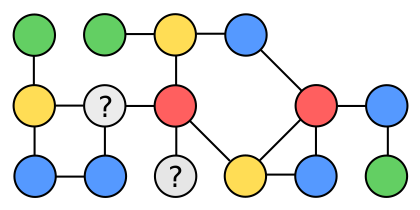
\includegraphics[width=0.4\linewidth]{images/VertexClassificationExample}
	\caption{Example of a graph with colors as vertex features.}
	\label{fig:vertexclassificationexample}
\end{figure}

A closer look reveals that, in this example, the color of a vertex corresponds to its degree. Thus $\text{deg}(v)$ may be a simple representation of each vertex $v$.

\paragraph{Example - Graph classification:} Consider the graph depicted in Figure \ref{fig:graphclassificationexample} and the task to predict the class of an unclassified graph (e.g. the gray one in the figure).
\begin{figure}[H] %TODO: Is this image TeXed? Lecture 0 Slide 30
	\centering
	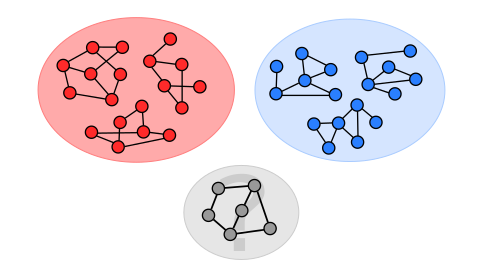
\includegraphics[width=0.5\linewidth]{images/GraphClassificationExample}
	\caption{Example of graph classification (clustering).}
	\label{fig:graphclassificationexample}
\end{figure}
A common approach is to use sets of subgraphs to describe (similarity between) graphs. In this example it appears that graphs of the red class contain cycles of length four whereas graphs of the blue class contain triangles. Thus, a graph $G$ may be represented by a vector $\phi(G)$ containing cycle counts of length three and four. 

\paragraph{Example - Link prediction:} Consider the graph depicted in Figure \ref{fig:linkpredictionexample} and the task to predict the likelihood of a not jet existing edge (e.g. the gray one in the figure).
\begin{figure}[H] %TODO: Is this image TeXed? Lecture 0 Slide 30
	\centering
	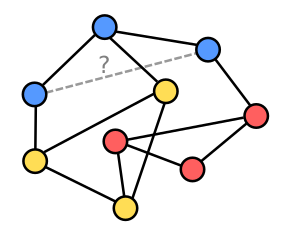
\includegraphics[width=0.4\linewidth]{images/LinkPredictionExample}
	\caption{Example of graph classification (clustering).}
	\label{fig:linkpredictionexample}
\end{figure}
A common approach is to consider the shortest path distance and similarity in terms of neighborhoods or vertex attributes. In this example the vertices of same color are more likely to be connected by an edge. Thus one may represent edges using the adjacent vertex colors.


As the given examples indicate, it can be tedious to analyze graph data and choose a suitable graph representation. As it turns out, Machine Learning can be used for learning the graph representations themselves. In the following chapter we will cover two aspects of graph representation learning:\begin{itemize}
	\item \textbf{Learning with representations} of graphs and
	\item \textbf{learning representations} of graphs.
\end{itemize}

%%%%%%%%%%%%%%%%%%%%%%%%%%%%%%%%%%
%%%%% Lecture 01 - 18.10.2021 %%%%
%%%%%%%%%%%%%%%%%%%%%%%%%%%%%%%%%%

\chapter{Vertex classifications and local features} %Learning vertex representations for graphs

\begin{Definition}[Directed graph]{def:DirectedGraph}
	A \textbf{directed graph} (\textbf{digraph}) $G=(V,E)$ consists of a set of vertices $V(G)$ and a set of edges $E(G) \subseteq V\times V$.
\end{Definition}

\begin{Definition}[Undirected Graph]{def:UndirectedGraph}
	A \textbf{undirected graph} $G=(V,E)$ consists of a set of vertices $V(G)$ and a set of edges $E(G) \subseteq 2^V$ such that
	\[ \forall e\in E(G):\qquad |e|=2 \]
\end{Definition}

As variable naming conventions, we say that graphs have $n=|V(G)|$ vertices and $m=|E(G)|$ edges.

\begin{Definition}[Simple graphs]{def:SimpleGraph}
	A simple graph is a graph, where edges connot appear multiple times.	
\end{Definition}

(That is, in the respective definitions of directed and undirected graphs, the set of edges is not a multiset.)

\begin{Definition}[Graph attributes and labels]{def:GraphAttributesLabels}
	Given an undirected or directed graph $G$, one can define additional data associated with the graph, vertices or edges. Such data is called \textbf{attributes} (if the value domain is continuous) or \textbf{labels} (if the value domain is discrete/categorical).
	
	This association can be formalized using \textbf{feature spaces} $\mathcal{X}$, $\mathcal{X}^\prime$ and $\mathcal{X}^{\prime\prime}$:
	\[ f_G: G \to \mathcal{X},\qquad\qquad f_V: V(G) \to \mathcal{X}^\prime,\qquad\qquad f_E : E(G) \to \mathcal{X}^{\prime \prime}\]
	(A feature space is some product space $\mathcal{X}=(X_1,X_2,\dots,X_d)$ where the $X_i$ are some appropriately chosen sets.)
\end{Definition}

\paragraph{Example - Graph labels} Typical examples of graph vertex labels are atom names (chemical graphs).

\begin{Definition}[Graph isomorphism]{def:GraphIsomorphism}
	Let $G$ and $H$ be two graphs. $G$ and $H$ are \textbf{isomorphic}, if and only if there exists a bijective function between the vertices $\varphi:V(G)\to V(H)$ such that
	\begin{itemize}
		\item edges are preserved:\\
		$ \{v,w\}\in E(G) \ \iff \ \{\varphi(v), \varphi(w)\}\in E(H) $
		\item vertex attributes are preserved:\\
		$ \forall v\in V(G):\ f_V(v) = f_V\big( \varphi(v)\big) $
		\item edge attributes are preserved:\\
		$ \forall \{v,w\}\in E(G):\ f_E(\{v,w\}) = f_E\big( \{ \varphi(v),\varphi(w) \} \big) $
	\end{itemize}
\end{Definition}

\section{Property prediction for vertices}

Learning functions (properties) on vertices is done under the assumption that there is a multiset of objects $X\subseteq \mathcal{X}$ and there exists an (partially) unknown function $y:X\to \mathcal{Y}$ and some pairs of objects are associated. This setting is formalized in definition \ref{def:SupervisedVPropPredition}.

\begin{Definition}[Supervised vertex property prediction on fixed graphs]{def:SupervisedVPropPredition}
	\vspace{-0.5cm}\begin{tabbing}
		\textbf{Output:} \= \kill
		\textbf{Input:} \>a graph $G$ with labeling functions $f_V$, $f_E$,\\
		\>a hypothesis class $\mathcal{H} \subseteq\{ h|\ h:V(G)\to \mathcal{Y} \}$,\\
		\>properties $y(v)$ for a set of vertices $v\in V^\prime \subseteq V(G)$ and\\
		\>a loss function $L_{V,y}:\mathcal{H}\to\IR$.\\
		\textbf{Output:} \>$\amin{h\in\mathcal{H}}{L_{V,y}}(h)$.
	\end{tabbing}
\end{Definition}

Note that one can extend hypothesis classes on graph vertices to their vertex representation. More explicitly, let $\mathcal{X}$ be a feature space and $r:V(G)\to \mathcal{X}$ some vertex representation on the graph $G$. Let $\mathcal{H}\subseteq \{ h|\ h:\mathcal{X}\to\mathcal{Y} \}$ be a hypothesis class. Then the \textit{extended hypothesis class} 
\begin{equation}
	\mathcal{H}^\prime := \{ h\circ r|\ h\in\mathcal{H} \}
\end{equation}
is a hypothesis class on $V(G)$, too.

On top of that one can generalize the vertex representation $r$ to a set of several graph representation $\mathcal{R}\subseteq \{r|\ r:V(G)\to\mathcal{X}\}$ and yield the further extended hypothesis class $\mathcal{H}^\prime := \{ h\circ r|\ r\in\mathcal{R},\ h\in\mathcal{H} \}$ on $V(G)$.

\subsection{Loss Functions - MERGE \& MOVE WITH THE STATISTIC SCRIPT} %TODO: MOVE TO THE STATISTIC SCRIPT

To measure the quality of hypothesis, with respect to vertex property predictions, one can use a variety of loss functions. Most of these can be generalized to other applications of hypothesis evaluation.

\begin{Definition}[Classification Loss]{def:ClassificationLoss}
	The \textbf{classification loss} of a hypothesis on vertices to predict their properties is defined as the probability of false predictions:
	\begin{equation}
		L_{V,y}(h) := \IP\big[ y(v) \neq h(v) \big] = 1-\frac{1}{|V(G)|} \sum_{v\in V(G)}\delta \big( y(v), h(v) \big)
	\end{equation}
	where 
	\[ \delta(a, b) = \begin{cases}
	1 & \text{if } a=b\\
	0 & \text{if } a\neq b
	\end{cases} \]
\end{Definition}

\begin{Definition}[Regression]{def:Regression}
	The \textbf{mean squared error} can be used as a loss function of a hypothesis on vertex property prediction. Using it to improve the quality of the found hypothesis is called \textbf{regression}:
	\begin{equation}
		L_{V,y}(h) := \IE\Big[ \big( y(x) -h(x)\big)^2 \Big] = \frac{1}{|V(G)|} \sum_{v\in V(G)} \big( y(v), h(v) \big)^2
	\end{equation}
\end{Definition}

When evaluating a (machine learning) model during training, we test a hypothesis on empirical data and optimize for the best solution. Both the optimization and the empirical data induce a bias on the estimate of the quality of the hypothesis. This bias can be reduced using \textbf{cross validation} (TODO - see Figure \ref). %TODO

\begin{figure}[H]
	\centering
	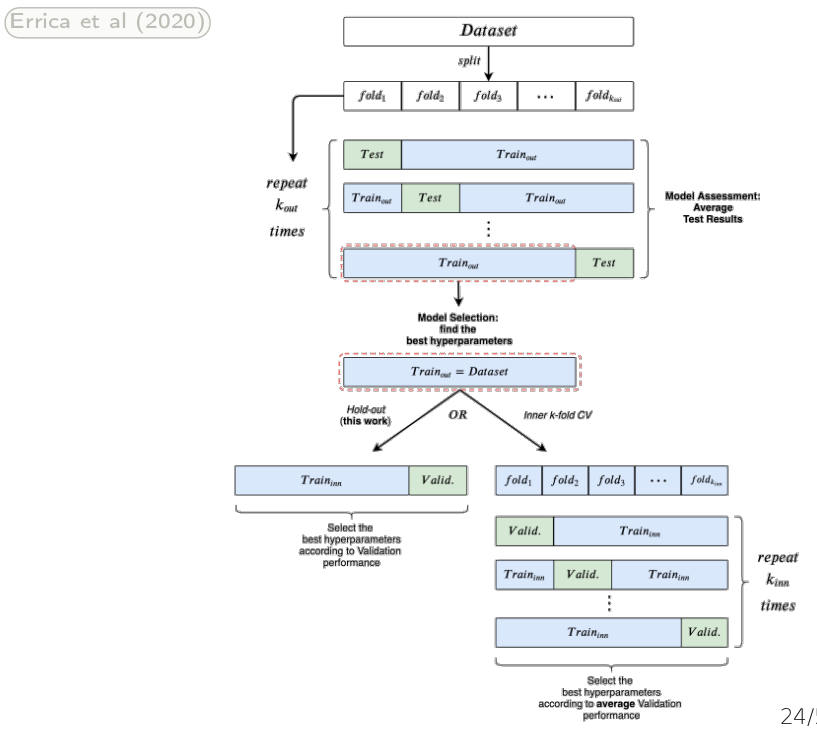
\includegraphics[width=0.7\linewidth]{images/crossvalidation}
	\caption{TODO: replace image} %TODO: replace image
	\label{fig:crossvalidation}
\end{figure}

Cross validation can be used to compare different hypothesis. If there is a statistically significant difference between their performances, one could be better than the other.

\subsection{Baselines for graph learning}

Interestingly, some baseline methods, which do not include specific graph structures may perform well, even better than GNNs on some graph datasets. In other words, improvements that do not clearly outperform structure-agnostic competitors should be viewed with moderation\cite{errica2019fair,schulz2019necessity,kriege2020survey,borgwardt2020graph}.

Note that whenever information about individual vertices is available, one should consider using it extensively. In many cases, it is more valuable for the task at hand, than the actual graph structure that combines these. 

To conclude, to evaluate a graph representation one should measure its performance against a model which ignores the graph structure. Thus when dealing with an attributed graph $G$ it can be beneficial to start with its vertex attributes $f_V: V(G)\to\mathcal{X}$ and first consider a hypothesis class over $\mathcal{X}$, only. Only after that, one may think about including graph representations into the hypothesis class.

\section{Local Feature Counts}

In this subsection we will define various simple vertex representations $f:V(G)\to\IR$ for fixed graphs. Let $\mathcal{R}^\prime$ be the set of all one-dimensional vertex representations. These representations can be grouped in the following way:
\begin{equation}
	\mathcal{R} := \{\times_R:V(G)\to\IR^{|R|}| \ R\subseteq \mathcal{R}^\prime\}
\end{equation}
where $\times_R(v)=\big( r_1(v), r_2(v),\dots, r_{|R|}(v) \big)$ for a vertex $v$ and representations $r_i\in R$.

\begin{Definition}[Vertex neighborhood]{def:VertexNeighborhood}
	Let $G$ be a undirected graph and $v\in V(G)$. The \textbf{neighborhood} of $v$ is the set
	\[ N(v):= \{w|\ \{v,w\}\in E(G)\} \]
	
	If $G$ is directed, we define respectively the \textbf{outgoind neighborhood} as 
	\[ N_{\text{out}}(v):= \{w|\ (v,w)\in E(G)\} \]
	and the \textbf{incoming neighborhood} as
	\[ N_{\text{in}}(v):= \{w|\ (w,v)\in E(G)\} \]
\end{Definition}

\begin{Theorem}[Full Neighborhood Representation]{thm:FullNeighborhoodRepresentation}
	By fixing an order of the vertices $V=\{ v_1,\dots,v_n \}$ and defining 
	\begin{equation}
	A(v_j)[i] :=\begin{cases}
	1 & \text{if }v_i\in N(v_k)\\
	0 & \text{if }v_i\notin N(v_k)
	\end{cases}
	\end{equation}
	one can represent a vertex by its neighborhood. This is called \textbf{Full Neighborhood Representation}.
\end{Theorem}

The drawbacks of a Full Neighborhood Representation include:\begin{itemize}
	\item The space requirements grow quadratically with $n$.
	\item Learning algorithms that use this representation will likely overfit.
	\item It requires additional effort to check, whether a given vertex is already included in the representation.
	\item It requires additional effort to find neighbors of neighbors.
\end{itemize}

The first two drawbacks can be reduced, by so called Compressed Neighborhood Representations. 

\begin{Definition}[Vertex degree]{def:VertexDegree}
	Let $G$ be a undirected graph and $v\in V(G)$ be a vertex. The \textbf{degree} is the number of edges incident to $v$, i.e.
	\[ \delta(v) := |N(v)| \]
	
	if $G$ is directed, we define respectively the \textbf{outdegree neighborhood} as the number of (incident) edges starting in $v$, i.e. 
	\[ \delta_{\text{out}}(v) := |N_{\text{out}}(v)| \]
	and the \textbf{indegree neighborhood} as the number of (incident) edges ending in $v$, i.e. 
	\[ \delta_{\text{out}}(v) := |N_{\text{out}}(v)| \]
\end{Definition}

The neighborhood $N(v)$ of a vertex $v$ induces a subgraph $G[N(v)]$ with the vertices in $N(v)$ and all edges between these vertices:
\[ G[N(v)] = \Big( N(v), \big\{\{w,w^\prime\}|\ w,w^\prime\in N(v) \big\} \Big) \]
The generalized definition is given in definition \ref{def:InducedSubgraph}.
This subgraph $G[N(v)]$ can have at most
\[ \frac{\delta(v)\big( \delta(v)-1 \big)}{2} \]
edges, since every of the $\delta(v)$ neighbors of $v$ can have at most one edge, to all other $\delta(v)$ neighbors in $G[N(v)]$. Notice, not to count every edge twice in this argumentation. If there are exactly this many edges (without loops), the subgraph is \textit{fully connected}.

\begin{Definition}[Neighborhood density\cite{watts1998collective,holland1971transitivity}] {def:NeighborhoodDensity}
	The \textbf{density} of a vertex's neighborhood $v$ is defined as the ratio of all existing edges and all possible edges (in a fully connected neighborhood):
	\[ c(v) := \frac{2 \big|E\big( G[N(v)] \big)\big|}{ \delta(v) \big(\delta(v)-1\big) } \]
\end{Definition}

\begin{Definition}[Induced subgraph]{def:InducedSubgraph}
	Let $G$ be a graph and $X\subseteq V(G)$ a set of its vertices. The \textbf{subgraph} of $G$ \textbf{induced by} $X$ is the graph $H$ with \begin{itemize}
		\item $V(H) = X$ and
		\item $E(H) = \big\{ \{v,w\}|\ \{v,w\}\in E(G)\ \land \ v,w\in X \big\}$
	\end{itemize}
\end{Definition}

A \textbf{triangle graph} is a simple graph on three vertices with three edges. 

\begin{Definition}[Triangle subgraphs]{def:TriangleSubraphCount}
	Let $\mathcal{D}(v)$ be the set of all triangle subgraphs of a graph $G$ that contain the vertex $v$.
	
	Let $\Delta(v) := |\mathcal{D}(v)|$ be its carnality.
\end{Definition}

\begin{Theorem}[Upper bound on the adjacent triangle count]{thm:AdjacentTriangleCount}
	Let $G$ be a graph and $v\in V(G)$. Then
	\[ \Delta(v) \le \big|E(G[N(v)])\big| \]
\end{Theorem}
\begin{Proof}
	Let $D\in\mathcal{D}(v)$ be an arbitrary triangle adjacent to $v \in V(G)$. Then $V(D) \subseteq N(v) \subseteq G[N(v)]$ since in a triangle all vertices are adjacent and thus all vertices in the triangle are adjacent to $v$ (i.e. contained in its neighborhood).
	
	Notice, that there are two kind of edges in $G[N(v)]$, the ones incident to $v$ ($v\in e$, there are $\delta(v)$ many of them) and these which are not ($v\notin e$). The ones incident to $v$ can be part of at most two triangles in $\Delta(v)$, while the edges that are not incident to $v$ can be part in exactly one triangle in $\Delta(v)$. That is because the two vertices that are adjacent to such an edge, together with $v$, completely define a triangle (if all edges are present).
	On the other hand, every triangle in $D(v)$ must contain exactly one edge, that is not incident to $v$ (and two which are incident to $v$).
	
	Therefore the number of triangles $\Delta(v)$ is equal to the number of edges in $G[N(v)]$ that are not incident to $v$, which is a fraction of all edges in $G[N(v)]$:
	\begin{flalign*}
		\Delta(v) &= \big|\{ e\in E(G[N(v)])| \ v\notin e\}\big| \\
		&\le \big|\{ e\in E(G[N(v)])| \ v\notin e\}\big| + \delta(v)\\
		&= \big|E(G[N(v)])\big|
	\end{flalign*}
	(Note that in the second equation, the equality is only achieved, if $v$ has no neighbors.)
\end{Proof}

\begin{Definition}[Induced Subgraph Isomorphism Problem]{def:InducedSubgraphIsoPb}
	\vspace{-0.5cm}\begin{tabbing}
		\textbf{Output:} \= \kill
		\textbf{Input:} \>two graphs $G$, $H$.\\
		\textbf{Output:} \>the decision if $H$ is isomorphic to an induced subgraph of $G$.
	\end{tabbing}
\end{Definition}

\begin{Theorem}[Difficulty of the Ind. Subgraph Iso. Pb.]{def:NPCompletenessOfInducedSubgraphIsoPb}
	The induced subgraph isomorphism problem is \textbf{NP-complete}.
\end{Theorem}
\begin{Proof}
	Let $K_n$ be a complete graph on $n$ vertices. Then solving the induced subgraph isomorphism problem for $K_n$ and $G$ solves the $k$-Clique Problem for $G$, which is NP-complete itself.
\end{Proof}

Notice, that if one could count the induced subgraphs for two graphs efficiently, one could decide the induced subgraph isomorphism problem. Hence \textit{counting induced subgraphs is NP-hard}.

But if one keeps the size of the induced subgraphs fix, the problem becomes tractable. 

\subsection{Graphlet Counting}

\begin{Definition}[Graphlet]{def:Graphlet}
	Small connected induced subgraphs are called \textbf{graphlets}.
\end{Definition}

We would like to count, for each vertex $v$, the number of graphlets of a certain type, that contain $v$. Lets call these $v$\textbf{-incident graphlets}.

\begin{Definition}[Incident Induced Graphlets Count Problem]{def:InducedSubgraphIsoPb}
	\vspace{-0.5cm}\begin{tabbing}
		\textbf{Output:} \= \kill
		\textbf{Input:} \>a graph $G$ and\\ 
		\>a graphlet $H$ of size $k$.\\
		\textbf{Output:} \>the number of $v$-incident induced subgraphs isomorphic to $H$ for all $v\in V(G)$:\\
		\>$ r_H(v) := \big|\{ X\subseteq V| \ v\in X\ \land\ G[X] \stackrel{\text{iso.}}{\equiv} H \}\big| $
	\end{tabbing}
\end{Definition}

\begin{algorithm}[H]
	\caption{Brute Force - Counting Incident Graphlets} \label{alg:BruteForceCountingIncidentGraphlets} 
	\begin{tabbing}
		\textbf{Output:} \= \kill
		\textbf{Input:} \>a graph $G$ and\\ 
		\>a graphlet $H$ of size $k$.\\
		\textbf{Output:} \>the number of $v$-incident induced subgraphs isomorphic to $H$ for all $v\in V(G)$.
	\end{tabbing}	
	\begin{algorithmic}[1]		
		\State $\text{gc}(v)=0$ for all $v\in V(G)$
		\For {\textbf{all} $X\subseteq V(G)$ with $|X|=k$}
			\If{$G[X]$ is isomorphic to $H$}
				\State $\text{gc}(x) = \text{gc}(x)+1$ for all $x\in X$
			\EndIf
		\EndFor
	\end{algorithmic}
	\textbf{Runtime}: There are ${n\choose k}$ choices for $X$, and there need $\gamma(k)\in \mathcal{O}( k! \ k^2)$ graphs to be checked for isomorphism. Thus the total runtime for a constant $k$ is
	\[ \mathcal{O} \big( n^k \ \gamma(k) \big) = \mathcal{O}(n^k)\]	
\end{algorithm}

Since a lot of graph structured data can be considered Big Data (w.r.t. size; not speed), cubic runtime in the number of vertices is not acceptable.

%%%%%%%%%%%%%%%%%%%%%%%%%%%%%%%%%%
%%%%% Lecture 02 - 25.10.2021 %%%%
%%%%%%%%%%%%%%%%%%%%%%%%%%%%%%%%%%

\begin{Theorem}[Runtime bound on the Incident Induced Graphlets Count Problem\cite{shervashidze2009efficient}]{thm:RuntimeBoundIncIndGraphletsCountPb}
	Let $G$ be a bounded degree graph and let $d$ denote the maximum degree in $G$. 
	
	If all graphlet structures size $k\in \{ 3, 4, 5 \}$ are known (precomputed), then all $v$-incident graphlets of $G$ with size $k\in \{ 3, 4, 5 \}$ can be enumerated in $\mathcal{O}(nd^{k-1})$ time.
\end{Theorem}
Notice that the maximum degree $d$ of a graph is typically much smaller than the number of its vertices $n$.
\begin{Proof}
	Graphlets of size $k$ can be divided into two classes:\begin{enumerate}
		\item Graphlets that contain a simple path of length $k-1$ and
		\item Graphlets that to not contain such a path.
	\end{enumerate}
	First, lets consider graphlets with paths of length $k-1$ and one fixed vertex $v\in V(G)$. We can enumerate all such paths in $G$ starting from $v$ by a depth-first search in $\mathcal{O}(d^{k-1})$.
	
	Each such path $P$ induces a subgraph $G[V(P)]$ containing $v$, which we can construct in $\mathcal{O}(k^2)$ time using appropriate data structures. 
	
	We can find the graphlet that $G[V(P)]$ is isomorphic to in $\gamma(k)\in\mathcal{O}(k!\ k^2)$ time and increase its count for $v$:\begin{itemize}
		\item Consider all $k!$ permutations of the vertex set of $G[V(P)]$ and
		\item check if the resulting adjacency matrix is identical to one of our precomputed graphlets ($\mathcal{O}(k^2)$, there are less than 30 of them).
	\end{itemize}
	Notice, that this approach has a couple of drawbacks:\begin{enumerate}
		\item If a graphlet may contain more than one path of length $k-1$, it will be counted/found multiple times!
		\item If $v$ is only in the middle of a path of length $k-1$ including graphlet, not graphlets that contain $v$ are found!
	\end{enumerate}
	There exist a solution for these drawbacks: Let $G[X]$ be a graphlet and $|X|=k$. Each $k-1$ path inducing $G[X]$ will be found exactly twice, one starting from each endpoint $v\neq v^\prime$. Thus we will find $G[X]$ twice for each $k-1$ path in it. Thus increasing a counter for each $w\in X$ each time we find $G[X]$ will yield a final count of 
		\[ 2\#(k-1 \text{ paths in }G[X]) \]
\end{Proof}

	%TODO: CONTINUE - Slide 16/59 ...

\begin{algorithm}[H]
	\caption{Exact Graphlet Counting Algorithm} \label{alg:ExactGraphletCountingAlg} 
	\begin{tabbing}
		\textbf{Output:} \= \kill
		\textbf{Input:} \>a graph $G$ and\\ 
		\>a graphlet $H$ of size $k$ and $1\le p$ paths of length $k-1$.\\
		\textbf{Output:} \>the number of $v$-incident subgraphs  isomorphic to $H$ for all $v\in V(G)$.
	\end{tabbing}	
	\begin{algorithmic}[1]		
		\State $\text{gc}(v)=0$ for all $v\in V(G)$
		\For {\textbf{all} $v \in V(G)$}
			\For {\textbf{all} $k-1$ length paths $P$ in $G$ starting in $v$}
				\If{$G[V(P)]$ is isomorphic to $H$}
					\State $\text{gc}(x) = \text{gc}(x)+1$ for all $x\in X$
				\EndIf
			\EndFor
		\EndFor
		\For {\textbf{all} $v\in V(G)$}
			$\text{gc}(v) = \frac{\text{gc}(v)}{2p}$ \Comment{B.c. of double counting}
		\EndFor
	\end{algorithmic} 
\end{algorithm}

To understand the runtime complexity, we need to consider how many graphlets without paths of length $k-1$ here are.\begin{itemize}
	\item[For $k=2$] There are no such graphlets.
	\item[For $k=3$] There are no such graphlets.
	\item[For $k=4$] There is only the $3$-star.\\
	We need to lookup all $\mathcal{O}\big({d\choose 3}\big)$ neighbor triplets of $v$ and check if they induce the $3$-star graphlet. This can be done in $\mathcal{O}(d^3 \gamma(4))$.
	\item[Fpr $k=5$] All connected graphlets with no $4$-paths have the $3$-star as subgraph.\\
	Thus enumerate all occurrences of the $3$-star and check the neighbors of each vertex (in the star) to see if they induce one of the graphlets. This takes $\mathcal{O}(d\gamma(5))$ per induced graph.
\end{itemize}
Thus the overall runtime is $\mathcal{O}(d^4\gamma(5))$.

Now, considering the relevance of the $3$-star we notice that since it has only one center, they cannot be found twice. Thus one may think, that the normalization step of the counter can be avoided.

However, the counts for graphlets of size five need to be normalized by the number of subgraphs of the pattern that are isomorphic to the $3$-star. Lets use this knowledge in another version of the algorithm.

\begin{algorithm}[H]
	\caption{Exact Graphlet Counting Algorithm 2} \label{alg:ExactGraphletCountingAlg2} 
	\begin{tabbing}
		\textbf{Output:} \= \kill
		\textbf{Input:} \>a graph $G$ and\\ 
		\>the $3$-star $H$.\\
		\textbf{Output:} \>the number of $v$-incident subgraphs  isomorphic to $H$ for all $v\in V(G)$.
	\end{tabbing}	
	\begin{algorithmic}[1]		
		\State $\text{gc}(v)=0$ for all $v\in V(G)$
		\For {\textbf{all} $v \in V(G)$}
			\For {\textbf{all} $X\subseteq N(v)$ with $|X|=3$}
				\If{$G[X\cup\{v\}]$ is isomorphic to $H$}
					\State $\text{gc}(x) = \text{gc}(x)+1$ for all $x\in X\cup\{v\}$
				\EndIf
			\EndFor
		\EndFor
	\end{algorithmic}
	\textbf{Runtime:} For pattern $H$ with $|V(H)|=k$ the runtime is $\mathcal{O}(nd^{k-1})$\\
	Repeating this for the set $\mathcal{G}_{3,4,5}$ for all 29 pairwise non-isomorphic graphs of size $k=3, 4, 5$ is also in $\mathcal{O}(nd^{k-1})$.\\
\end{algorithm}

\begin{algorithm}[H]
	\caption{Exact Graphlet Counting Algorithm 3} \label{alg:ExactGraphletCountingAlg3} 
	\begin{tabbing}
		\textbf{Output:} \= \kill
		\textbf{Input:} \>a graph $G$ and\\ 
		\>the $3$-star $H$ of size $5$ without simple $k-1$ length paths and $1\le x$ $3$-stars.\\
		\textbf{Output:} \>the number of $v$-incident subgraphs  isomorphic to $H$ for all $v\in V(G)$.
	\end{tabbing}	
	\begin{algorithmic}[1]		
		\State $\text{gc}(v)=0$ for all $v\in V(G)$
		\For {\textbf{all} $v \in V(G)$}
			\For {\textbf{all} $X\subseteq N(v)$ with $|X|=3$}
				\If{$G[X\cup\{v\}]$ is isomorphic to $H$}
					\For{$w\in \bigcup_{x\in X\cup\{v\}}N(x)$} 
						\If {$H$ is isomorphic to $G[X\cup\{v,w\}]$}
							\State $\text{gc}(x) = \text{gc}(x)+1$ for all $x\in X\cup\{v,w\}$
						\EndIf
					\EndFor
				\EndIf
			\EndFor
		\EndFor
		\For {\textbf{all} $v\in V(G)$}
			$\text{gc}(v) = \frac{\text{gc}(v)}{2p}$ \Comment{B.c. of double counting}
		\EndFor
	\end{algorithmic}
	\textbf{Runtime:} For pattern $H$ with $|V(H)|=k$ the runtime is $\mathcal{O}(nd^{k-1})$\\
	Repeating this for the set $\mathcal{G}_{3,4,5}$ for all 29 pairwise non-isomorphic graphs of size $k=3, 4, 5$ is also in $\mathcal{O}(nd^{k-1})$.\\
\end{algorithm}

(Note that in practice the order of the loops should be changed.)

With these algorithms at hand, we can proclaim that for all $H\in\mathcal{G}_{3,4,5}$ we can efficiently compute
\[ r_H(v) \ := \ |\{ X\subseteq V| \ v\in X\land G[X] \text{ is isomorphic to }H \}| \]
and hence we can efficiently compute the representation of graphs by $2, 3, 4, 5$-graphlets:
\begin{equation}\label{eq:GraphletGraphRepresentation}
	\times_{\{r_H|\ H\in\mathcal{G}_{2,3,4,5}\}}: V(G) \to \IR^{29}
\end{equation}



One may ask, how significant the runtime improvement from $\mathcal{O}(n^k)$ in Algorithm \ref{alg:BruteForceCountingIncidentGraphlets} to $\mathcal{O}(nd^{k-1})$ in Algorithm \ref{alg:ExactGraphletCountingAlg3} really is. As it turns out this improvement is the change between an impractical and a practical algorithm since in the latter only connected subgraphs considered, which is as desired. Im most real world graphs, there are much less such connected sets than there are subsets.

One may also ask, how significant these results are, given that we only considered small graphlets. As it turns out, in many databases these small graphlets can be interpreted more easily than bigger ones. For example in social networks, many triangle graphlets may indicate that friends of friends tend to be friends as well. While many 2-paths imply the opposite. Nevertheless, larger graphlets can be useful in practice too.

Keep in mind, that so far we considered unlabeled graphs. Taking labels into account yields much more pairwise non-isomorphic graphs. Note that in practice, graphlet counting (and multiple other pattern based representation methods) tends to \textit{work better with discretely labeled attributes} than with continuous attributes (e.g. $f_V:V(G)\to\IR$). Thus it may be desirable to discretize given continuous labels.

\section{Distance based vertex representations}

We have seen that graphlet counting (as an example of local feature counting) extends the trivial neighborhood set representation to the immediate neighborhood. But it to does not go beyond a few neighbors.

\subsection{Centrality measures with distances}

\begin{Definition}[Geodesic graph distance]{def:GeodesicGraphDistance}
	Let $G$ be a graph and $v, w\in V(G)$. Then the (\textbf{geodesic}) \textbf{distance} $d(v,w)$ is the length of the \textbf{shortest path} in $G$ with $v$ and $w$ as its endpoints.
	
	
	More explicitly, the \textbf{unweighted} (\textbf{geodesic}) \textbf{distance} is the number of edges in the path. On the other hand the \textbf{weighted} (\textbf{geodesic}) \textbf{distance} for some weight function $c:E(G)\to\IR_{\ge 0}$ is the sum of weights of edges in this path.
	
	If such a path between $v$ and $w$ does not exist, set $d(v,w) := \infty$.
\end{Definition}

A trivial but expensive approach to represent the graph structure is to compute and store all distances to all other vertices in the graph. This has time complexity \begin{itemize}
	\item $\mathcal{O}(nm)$ using BFS for \textit{unweighted} graphs and
	\item $\mathcal{O}(n^2 \log(n)+nm)$ using Johnsons algorithm for \textit{weighted} graphs
\end{itemize}
and space complexity $\Theta(n^2)$. For many (big) real world graphs this is infeasible.

\begin{Definition}[(Vertex) closeness centrality]{def:VertexClosenessCentrality}
	Let $G$ be a connected graph and $v\in V(G)$. The \textbf{closeness centrality} of $v$ is defined as
	\begin{equation}
		C_{\text{c}}(v) := \begin{cases}
			\infty & \text{if $G$ is disconnected}\\
			0 & \text{if $G$ has only one vertex}\\
			\frac{n-1}{\sum_{w\in V(G)\backslash\{v\}} d(v,w) } & \text{else}
		\end{cases}
	\end{equation}
	That is the ratio of the distance of all vertices to $v$, if $v$ would be connected to every vertex - and the actual accumulated distances to all vertices.
\end{Definition}

\begin{minipage}{\textwidth}
	\begin{figure}[H]
		\centering
		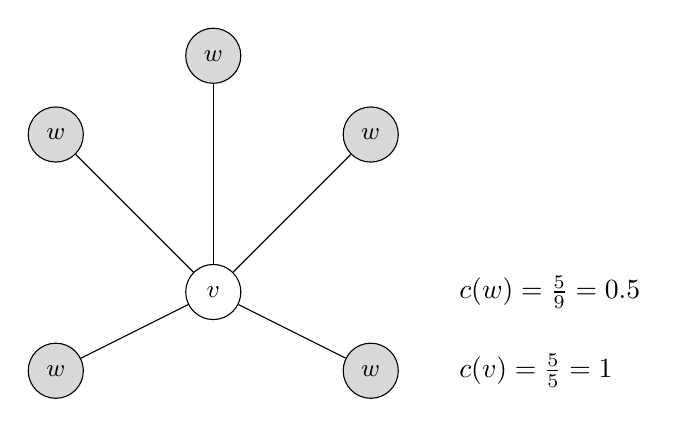
\begin{tikzpicture}[x=2cm,y=2cm] 
		\begin{scope}[scale=1]
		
		\tikzstyle{mycircle}=[circle,
		draw=black,
		fill=gray,
		fill opacity = 0.3,
		text opacity=1,
		inner sep=0pt,
		minimum size=7mm,
		font=\small
		]
		\tikzstyle{mycirclewhite}=[circle,
		draw=black,
		text opacity=1,
		inner sep=0pt,
		minimum size=7mm,
		font=\small
		]
		
		\coordinate (px1) at (1, 3.5);
		
		\coordinate (px2) at (0, 3);
		\coordinate (px3) at (2, 3);
		\coordinate (px4) at (1, 2);
		
		\coordinate (px5) at (0, 1.5);
		\coordinate (px6) at (2, 1.5);
		
		\coordinate (t1) at (2.5, 1.5);
		\coordinate (t2) at (2.5, 2);
		
		
		\node[mycircle] (x1) at (px1) {$w$};	
		\node[mycircle] (x2) at (px2) {$w$};
		\node[mycircle] (x3) at (px3) {$w$};	
		\node[mycirclewhite] (x4) at (px4) {$v$};
		\node[mycircle] (x5) at (px5) {$w$};	
		\node[mycircle] (x6) at (px6) {$w$};
		
		
		\draw[-] (x1) -- (x4);
		\draw[-] (x2) -- (x4);
		\draw[-] (x3) -- (x4);
		\draw[-] (x5) -- (x4);
		\draw[-] (x6) -- (x4);
		

		\draw[] (t1) node[right] {$c(v) = \frac{5}{5} = 1$};
		\draw[] (t2) node[right] {$c(w) = \frac{5}{9} = 0.5$};
		
		\end{scope}
		\end{tikzpicture}
	\end{figure}
	\captionof{figure}{Example for the closeness centrality measure}
	\label{fig:closenesscentrality2}
\end{minipage}

Note that this closeness centrality is a well-known centrality measure. A scaled version of it is used for example in the k-means cluster reassignment step. There one is optimizing with respect to the accumulated pairwise Euclidean distance:
\[ \amin{x\in \IR^2}\sum_{y\in C_i} L_2^2(x,y) \ = \amax{x\in \IR^2} \frac{1}{ \sum_{y\in C_i} L_2^2(x,y) } \ = \amax{x\in \IR^2} \frac{n-1}{ \sum_{y\in C_i} L_2^2(x,y) }\]

\begin{Definition}[Harmonic closeness centrality]{def:HarmonicClosenessCentrality}
	Let $G$ be a graph and $v\in V(G)$. The \textbf{harmonic closeness centrality} of $v$ is
	\begin{equation}
		C_{\text{hc}}(v) := \frac{1}{n-1} \sum_{w\in V(G)\backslash\{v\}} \frac{1}{d(v,w)}
	\end{equation}
	while defining $\frac{n-1}{\infty} := 0$.\\
	
	Thus $C_{\text{hc}}$ is well defined on disconnected graphs and again zero if there is only one vertex in $G$.
\end{Definition}

\begin{minipage}{\textwidth}
	\begin{figure}[H]
		\centering
		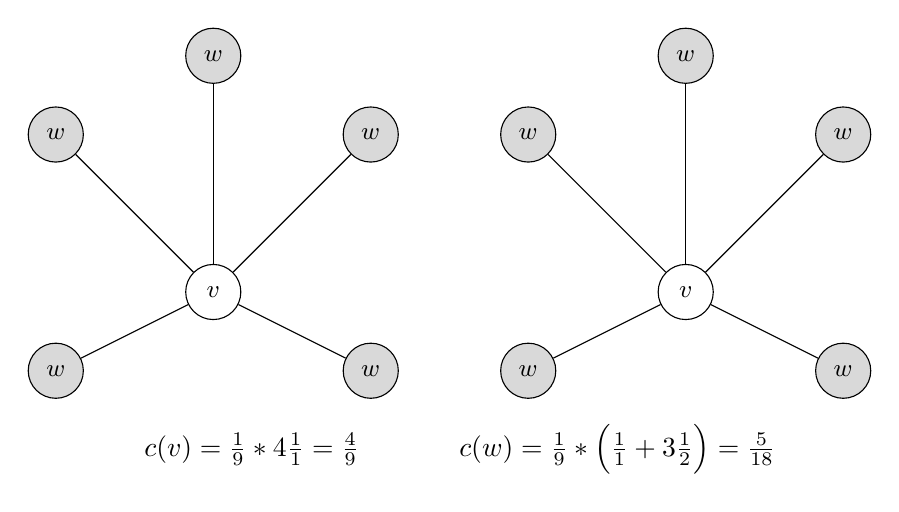
\begin{tikzpicture}[x=2cm,y=2cm] 
		\begin{scope}[scale=1]
		
		\tikzstyle{mycircle}=[circle,
		draw=black,
		fill=gray,
		fill opacity = 0.3,
		text opacity=1,
		inner sep=0pt,
		minimum size=7mm,
		font=\small
		]
		\tikzstyle{mycirclewhite}=[circle,
		draw=black,
		text opacity=1,
		inner sep=0pt,
		minimum size=7mm,
		font=\small
		]
		
		\coordinate (px1) at (1, 3.5);		
		\coordinate (px2) at (0, 3);
		\coordinate (px3) at (2, 3);
		\coordinate (px4) at (1, 2);		
		\coordinate (px5) at (0, 1.5);
		\coordinate (px6) at (2, 1.5);
		
		\coordinate (t1) at (0.5, 1);
		\coordinate (t2) at (2.5, 1);
		
		\node[mycircle] (x1) at (px1) {$w$};	
		\node[mycircle] (x2) at (px2) {$w$};
		\node[mycircle] (x3) at (px3) {$w$};	
		\node[mycirclewhite] (x4) at (px4) {$v$};
		\node[mycircle] (x5) at (px5) {$w$};	
		\node[mycircle] (x6) at (px6) {$w$};
				
		\draw[-] (x1) -- (x4);
		\draw[-] (x2) -- (x4);
		\draw[-] (x3) -- (x4);
		\draw[-] (x5) -- (x4);
		\draw[-] (x6) -- (x4);
		
		
		\coordinate (py1) at (4, 3.5);		
		\coordinate (py2) at (3, 3);
		\coordinate (py3) at (5, 3);
		\coordinate (py4) at (4, 2);		
		\coordinate (py5) at (3, 1.5);
		\coordinate (py6) at (5, 1.5);		
		
		\node[mycircle] (y1) at (py1) {$w$};	
		\node[mycircle] (y2) at (py2) {$w$};
		\node[mycircle] (y3) at (py3) {$w$};	
		\node[mycirclewhite] (y4) at (py4) {$v$};
		\node[mycircle] (y5) at (py5) {$w$};	
		\node[mycircle] (y6) at (py6) {$w$};
		
		\draw[-] (y1) -- (y4);
		\draw[-] (y2) -- (y4);
		\draw[-] (y3) -- (y4);
		\draw[-] (y5) -- (y4);
		\draw[-] (y6) -- (y4);
				
		\draw[] (t1) node[right] {$c(v) = \frac{1}{9}*4\frac{1}{1} = \frac{4}{9}$};
		\draw[] (t2) node[right] {$c(w) = \frac{1}{9}*\Big( \frac{1}{1}+ 3 \frac{1}{2} \Big) = \frac{5}{18}$};
		
		\end{scope}
		\end{tikzpicture}
	\end{figure}
	\captionof{figure}{Example for the closeness centrality measure}
	\label{fig:closenesscentrality}
\end{minipage}

Unfortunately, no algorithm is known to compute the closeness centrality for all vertices faster than by trivially computing all-pairs-shortest paths. This is possible in $\mathcal{O}(n^2 \log(n)+nm)$ in the weighted case.

\begin{Definition}[Sampled harmonic closeness centrality]{def:SampledHarmonicClosenessCentrality}
	Let $G$ be a graph, $v\in V(G)$ and $L\subseteq V(G)$. The \textbf{sampled harmonic closeness centrality} of $v$ with respect to $L$ is
	\begin{equation}
	C_{\text{hc},L}(v) := \frac{1}{|L\backslash\{v\}|} \sum_{w\in L\backslash\{v\}} \frac{1}{d(v,w)}
	\end{equation}
	while defining $\frac{|L|}{\infty} := 0$.\\
	
	This is the harmonic closeness centrality, limited to a subset $L$ of vertices of the graph.
\end{Definition}

The sampled harmonic closeness centrality for all vertices an be computed in $\mathcal{O}\big(|L|(m+n\log(n))\big)$ by running Dijkstras algorithm starting from each vertex $l\in L$, which we call \textbf{landmarks}. This approach can be implemented to have $\mathcal{O}(n)$ space complexity (in addition to storing the graph itself).

Similar to the graphlet graph representation equation \ref{eq:GraphletGraphRepresentation} we can express the representation in terms of these landmarks:
\begin{equation}\label{eq:LandmarksGraphRepresentation}
	\times_{\{d_l|\ l\in L\}}: V(G) \to \IR^{|L|}
\end{equation}

A real life interpretation of this sampled harmonic closeness would be to define ones position by saying: \enquote{I am 1 km way from the university and 500 m way from the church.} The usefulness of this description depends on the selected landmarks $L$ of course. There is no generally optimal strategy to select them. Some example approaches are:\begin{itemize}
	\item random initialization
	\item high-degree graph vertices
	\item in 2D-embedded (planar) graphs, use vertices on the convex hull
	\item vertices with high (or low) closeness centrality
	\item informed choice: cover the graph such that most vertices have at least one landmark close by
\end{itemize}

\subsection{Centrality measures without distances}

The sampled closeness centrality proposed in the last subsection might not be good enough. On the other hand, more exact closeness computations are easily to expensive. On top of that, in some graphs, all vertices might be almost equally central (curse of dimensionality). Thus in this subsection we will explore alternatives to distances.

\subsubsection{Degeneracy}

Another way of defining centrality is via \textit{density}. Intuitively, it would make sense for a graph to have a dense core and a sparse shell. To be efficient, one has to be careful to not solve the Clique problem along the way.

\begin{Definition}[Vertex degree]{def:VertexDegree}
	Let $G$ be a graph and $H$ be a subgraph of $G$. For $v\in V(H) \subseteq V(G)$ we denote the degree of $v$ in $H$ by $\delta_H(v)$.
\end{Definition}

\begin{Definition}[$k$-core component of a graph]{def:kCoreComponent}
	A $k$\textbf{-core component} of a graph $G$ is an inclusion-wise maximal connected induced subgraph $G[X]$ such that each vertex $x\in X$ has at least degree $k$ in the induces subgraph
	\[ \delta_{G[X]}(x) \ge k \]
\end{Definition}

\begin{Definition}[$k$-core of a graph]{def:kCoreOfGraphs}
	The subgraph $H(k)$ of $G$ consisting of all $k$-core components is called the $k$\textbf{-core of} $G$.
\end{Definition}

\begin{Definition}[Degeneracy]{def:degeneracy}
	The \textbf{degeneracy} $\text{deg}(v)$ of $v\in V(G)$ is the largest $k$ such that $v$ is contained in the $k$-core of $G$.
\end{Definition}

\begin{figure}[H]
	\centering
	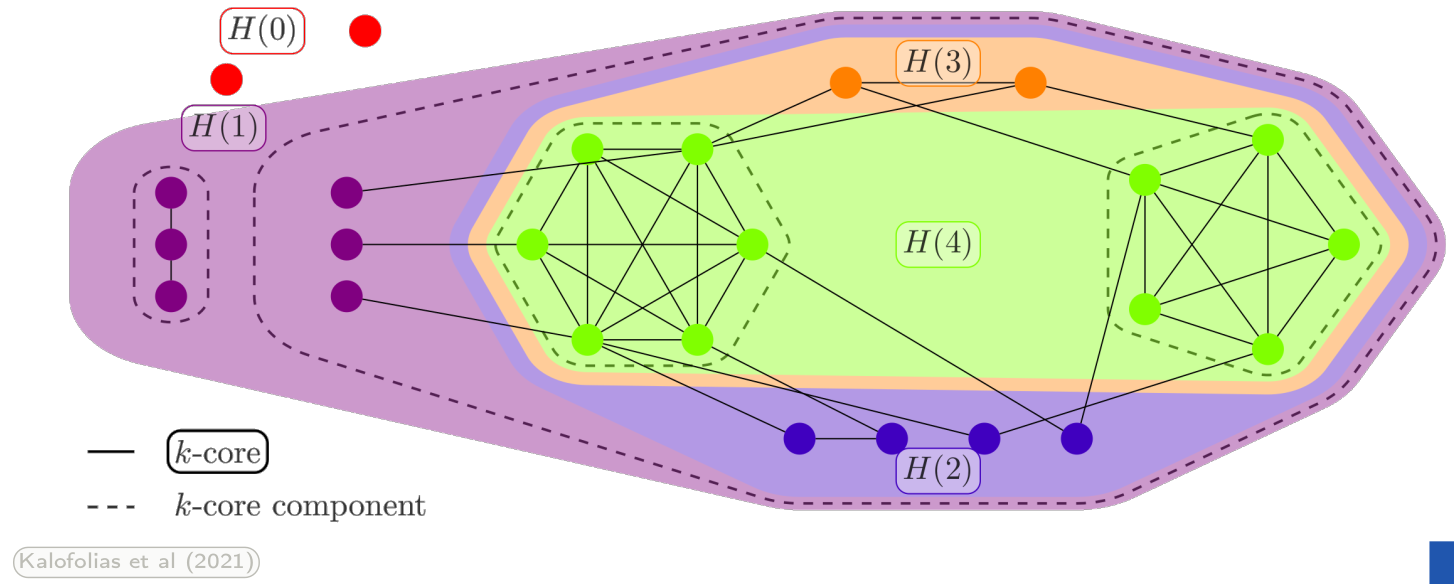
\includegraphics[width=\linewidth]{images/degeneracyExample}
	\caption{Example graph with all $k$-cores and thus degeneracies visualized\cite{kalofolias2021susan}.}
	\label{fig:degeneracyexample} %TODO: Get code from pascal
\end{figure}

\begin{Definition}[Smallest first vertex ordering]{def:SmallestFirstVertexOrdering}
	The vertices $v_1,\dots, v_n$ of $G$ are in \textbf{smallest first ordering} if for all $i\in \{1,\dots, n\}$ holds:
	\begin{center}
		$v_i$ is the vertex with smallest degree in $G\big[ \{ v_i,\dots, v_n \} \big]$
	\end{center}
\end{Definition}

\begin{algorithm}[H]
	\caption{Degeneracy sweep} \label{alg:Degeneracy} 
	\begin{tabbing}
		\textbf{Output:} \= \kill
		\textbf{Input:} \>a graph $G$.\\
		\textbf{Output:} \>the degeneracies $\text{deg}$ of all vertices $v\in V(G)$.
	\end{tabbing}	
	\begin{algorithmic}[1]		
		\State $k=0$
		\For {$i\in\{1,\dots,n\}$}
			\State Remove $v \:= \amin{v\in V} d_{\min}$ and all incident edges from $G$
			\State $k = \max(d_{\min}, k)$ \label{line:degeneracyLowerBound}
			\State $\text{deg}(v)=k$ \label{line:degeneracyUpdate}
		\EndFor
	\end{algorithmic}
	\textbf{Runtime}: $\mathcal{O}(n)$.\\
	\textbf{Special property:} The algorithm processes the vertices in smallest first vertex order.
\end{algorithm}


\begin{Theorem}[Complexity of degeneracy\cite{matula1983smallest}]{thm:ComplexityOfDegeneracy}
	Let $G$ be a graph. The degeneracy of all vertices $v\in V(G)$ can be computed in linear time.
\end{Theorem}
\begin{Proof}
	We have proven the claim if algorithm \ref{alg:Degeneracy} runs in linear time. Therefore we need to show that $\text{deg}(v)=k$ in line \ref{line:degeneracyUpdate} correctly computes the degeneracy of $v$ in each iteration, since every vertex is touched exactly once in the for loop.
	
	Let $v_1,\dots,v_n$ be the smallest first vertex order used by the algorithm. Let $d_i := \delta_{G\big[ \{ v_i,\dots,v_n \} \big]}(v_i)$. Then 
	\begin{equation}
		\forall i\in\{1,\dots,n \}:\qquad \delta_{G\big[ \{ v_i,\dots,v_n \} \big]}(v) \ge d_i
	\end{equation}
	That is, $G\big[ \{ v_i,\dots,v_n \} \big]$ is a subgraph of the $d_i$-core of $G$.
	
	This also implies that $G\big[ \{ v_i,\dots,v_n \} \big]$ is a subgraph of the $d_j$-core for all $1\le j\le i$.
	
	Hence, line \ref{line:degeneracyLowerBound} of the algorithm sets a lower bound on the degeneracy of each vertex coming after the current one in the smallest first ordering.
	
	Now let $H$ ba a $k$-core component in $G$ and let $v_1,\dots, v_n$ be any smallest first ordering. Let $i$ be the smallest index with $v_i\in V(H)$. We claim that it is $d_i\ge k$. To se this note that as $V(H) \subseteq \{ v_i,\dots, v_n \}$, $H$ is a subgraph of $G\big[ \{v_i,\dots, v_n\} \big]$. This implies
	\[ d_i = \delta_{G\big[ \{ v_i,\dots,v_n \} \big]}(v_i) \ge \delta_H(v_i) =k \]
	
	Thus line \ref{line:degeneracyLowerBound} of the algorithm also sets an upper bound on the degeneracy of each vertex. Thus the equality $d_i =k$ is proven.
\end{Proof}

With respect to the space complexity of Algorithm \ref{alg:Degeneracy} we note that in each iteration we have to find the remaining vertex with the smallest degree, remove it, and update the degrees of the (ex-)neighbors. We can do this in linear time using lists and arrays:
\begin{itemize}
	\item Store $G$ in a standard adjacency list format.
	\item In an array $A$, for each $\delta \in \{1,\dots, n\}$ store a \textbf{double linked list}, initialized with all vertices that have degree $i$.
	\item Om am array $B$, for each vertex, store its current degree and a pointer to its unique list entry maintained in $B$.
	\item Start with the first non-empty list in $A$, popping the first element $v$, decreasing the degrees of its neighbors by one in $B$, and moving them from their current list in $A$ to the list of their new degree (using the pointer in $B$ for constant time access to the list entries).	
	\item Continue looking for the first non-empty list in $A$, \textit{starting with the previous list} in $A$, checking if there is now a vertex with that degree.
\end{itemize}
Keep in mind that as $A$ contains double linked lists, removing and adding list items takes constant time.

%%%%%%%%%%%%%%%%%%%%%%%%%%%%%%%%%%
%%%%% Lecture 03 - 08.11.2021 %%%%
%%%%%%%%%%%%%%%%%%%%%%%%%%%%%%%%%%

\section{Message passing}

Note that the power set of a set $X$ can be denoted as $2^X$. Since multisets contain objects a non-negative number of times, the set of all multisets of objects from $X$ can be denotes as $\mathbb{N}^X$.

We will now introduce a very flexible framework. Assume that we have some feature representation $r_0 : V(G) \to \IR^d$ for the vertices in our graph. It is reasonable that in many situations neighboring vertices influence each other. Consider a social network where users spread their content along connections to their affiliates. In turn, neighbors might be influenced by that and hence spread (a variant of) that information (aka. \enquote{retweet}).

\textbf{Message passing} models this kind of behavior as a \textit{simultaneous round based process}:

\begin{Definition}[Message passing]{def:MessagePassing}
	\textbf{Message passing} models a simultaneous round based process. Let $v\in V(G)$ be a vertex, $k\ge 0$ and $r_0:V(G)\to \mathcal{X}_0$ a feature representation.
	
	$\mset{ r_k(w)| \ w\in N(v) }$ is the multiset of (old) representations of the neighbors of $v\in V(G)$. Define the following two functions:
	\begin{itemize}
		\item $\operatorname{agg}_k : \IN^{\mathcal{X}_k} \to\mathcal{X}_k^\prime$ \textbf{aggregates} a set of (old) representations to some value.
		\item $\operatorname{upd}_k : \mathcal{X}_k \times \mathcal{X}_k^\prime \to\mathcal{X}_{k+1}$ \textbf{updates} the representation of $v$ given its old representation and the aggregate of the neighbors.
	\end{itemize}
	Omit $k$ in the notation of $\operatorname{upd}_k$ and $\operatorname{agg}_k$ when the functions are iteration independent ($\operatorname{upd}_0 = \operatorname{upd}_1 = \dots$).
	
	With these notations message passing can be described as the following representation update:
	\begin{equation}\label{eq:MessagePassing}
		r_{k+1}(v) = \operatorname{upd}_k \Big( r_k(v), \operatorname{agg}_k \big(r_k(w)|\ w\in N(v)\big) \Big)
	\end{equation}
\end{Definition}

In practice, message passing is often used with $\mathcal{X}_0 = \mathcal{X}_0^\prime = \mathcal{X}_1 = \mathcal{X}_1^\prime  = \dots = \IR^d$ for some fixed $d$. Then the aggregation function $\operatorname{agg}:\IN^{IR^d}\to \IR^d$ a set of (old) representations to some value from the same domain. The update function is then of the form $\operatorname{upd}:\IR^d\times \IR^d \to\IR^d$.

Note that the definition of message passing depends on the multiset of neighbors of a vertex. Thus the order in which those neighbors are (practically) process does not influence the resulting representation of the central vertex. More general, the method is \textbf{invariant under isomorphism}:

\begin{Theorem}[Message passing is invariant under isomorphism] {thm:MessagePassingInvariantUnderIsom}
	Let $G$ and $H$ be two graphs and $r_0^G$ and $r_0^H$ two vertex representations with fixed aggregator and update functions:
	\begin{itemize}
		\item[] $r_1^G(v) = \operatorname{upd}\Big( r_0^G(v), \operatorname{agg}\big( \mset{ r_0^G(w)| \ w \in N(v) } \big) \Big)$
		\item[] $r_1^H(v) = \operatorname{upd}\Big( r_0^H(v), \operatorname{agg}\big( \mset{ r_0^H(w)| \ w \in N(v) } \big) \Big)$
	\end{itemize}	
	Let $\varphi :V(G) \to V(H)$ be an isomorphism that respects $r_0^G$ and $r_0^H$:
	\begin{equation}\label{eq:MessagePassingInvIsok0}
		r_0^G(v) = r_0^H(\varphi(v))
	\end{equation}
	
	Then message passing (the next iteration of the vertex representation) is invariant under isomorphism:
	\[ \forall k\ge 0: \qquad r_k^G(v) = r_k^H\big( \varphi(v) \big) \]
\end{Theorem}
\begin{Proof}
	The case $k=0$ is true by definition of $\varphi$ (equation \ref{eq:MessagePassingInvIsok0}). First lets prove $k=1$. Let $v\in V(G)$. We will use the preserved neighborhoods under isomorphism
	\begin{equation}\label{eq:NeighborhoodsUnderIso}
		w\in N(v) \iff \varphi(w)\in N\big(\varphi(v)\big)
	\end{equation}
	and the following equality of multisets (using again equation \ref{eq:MessagePassingInvIsok0}):
	\begin{flalign}\label{eq:MultisetIsoEqualities}
		\mset{ r_0^G (w)|\ w\in N(v) } 
		&= \mset{ r_0^H (\varphi(w))|\ \varphi(w)\in N(\varphi(v)) } \nonumber\\
		&=  \mset{ r_0^G (w^\prime)|\ w^\prime\in N(\varphi(v)) } 
	\end{flalign}

	Now it is:\begin{flalign*}
		r_1^G(v) &= \operatorname{upd}\Big( r_0^G(v), \ \operatorname{agg}\big( \mset{ r_0^G(w)|\ w\in N(v)} \big) \Big) && \text{by definition}\\
		&= \operatorname{upd}\Big( r_0^H(\varphi(v)), \ \operatorname{agg}\big( \mset{ r_0^G(w)|\ w\in N(v)} \big) \Big) && \text{using \ref{eq:MultisetIsoEqualities}}\\
		&= \operatorname{upd}\Big( r_0^H(\varphi(v)), \ \operatorname{agg}\big( \mset{ r_0^H(w^\prime)|\ w^\prime\in N(\varphi(v))} \big) \Big) && \text{using \ref{eq:NeighborhoodsUnderIso}}\\
		&= r_1^H(\varphi(v)) && \text{by definition}\\
	\end{flalign*}
	Now lets prove the statement for $k>1$.	%TODO: Prove message passing iso invaiance
\end{Proof}

We have just shown that the vertex representations computed by message passing do not depend on the order of the vertices. Note that instead of a multiset of neighbor representations, a set would work to.

Also note, that in iteration $k$ the representation of $v$ is determined by the (intermediate) representations of all vertices of distance at most $k$ from $v$, since more the neighborhood of the next iteration depends on its neighbors of the previous one.

\subsection{Aggregator functions}

Common choices for aggregator functions are: \begin{itemize}
	\item counts,
	\item means, sums, products, 
	\item histograms,
	\item hashes and
	\item Neural Networks.
\end{itemize}

Lets consider these aggregator functions one by one.

\subsubsection{Neighbor count aggregator}

Consider the \textbf{neighbor count aggregator}. Since the graph structure does not change, the multiset of neighbor representations of any vertex $v$ has constant size in each iteration. Thus the aggregator will, for each vertex, produce a \textbf{constant value} over all iterations of message passing. This is rather trivial.

\subsubsection{Means, sums and products aggregator}

One can also generalize the \textbf{means}, \textbf{sums} and \textbf{products aggregator} by defining a binary operation that is commutative and associative $\circ:\mathcal{X}\times \mathcal{X} \to \mathcal{X}$. For $X=\mset{ x_1,x_2,\dots,x_{|X|}}$
\[ \bigcirc_{x\in X} x = x_1\circ x_2 \circ \dots \circ x_{|X|} \]
is a well defined aggregator.

\subsubsection{Histogram aggregator}

Lets take a closer look at \textbf{histogram aggregators}. Let $\mathcal{X}$ be a set and $B_1, B_2,\dots, B_k\subseteq \mathcal{X}$ be bins. Then for $X\in \IN^{\mathcal{X}}$ and $B_i$ we can define
\[ \text{count}_{B_i} (X) := |\mset{ x\in X| \ x\in B_i }| \]
and $\text{hist}_{B_1,\dots,B_k}:\mathcal{X}\to \IN^k$ as
\[ \text{hist}_{B_1,\dots,B_k}(X) := \big( \text{count}_{B_1}(X),\dots, \text{count}_{B_k}(X) \big) \]
Note that the histograms generalize multisets, since a multiset is a histogram where each bin contains a single object. One can also define \textbf{weighted versions} where one sums over weights of objects in a bin.

While histograms are very useful, whey are not straightforwardly applicable to message passing.

\subsubsection{Hash aggregator}

We can define an aggregator that assigns each multiset an (ideally unique) identifier (hash).
Abstractly, we only require that $\#:\IN^{\mathcal{X}}\to \mathcal{X}^\prime$ is a function, i.e. that the same multiset will always be mapped to the same value.
If such a function is injective it is called a \textbf{perfect hash function}. There are multiple ways of implementing this in practice.

\subsubsection{Neural network aggregator}

We can use any Neural Network $f_{\phi}:\IN^{\IR^d}\to \IR^{d^\prime}$ that accepts a set of representations as input and produces an output. In the simplest case, one can use a Perceptron with indegree equal to the maximum degree of the graph times $d$. One has to be careful to have a permutation invariant function, though.

\subsection{Update functions}

The update function $\operatorname{upd}:\mathcal{X}_k \times\mathcal{X}_k^\prime \to \mathcal{X}_{k+1}$ updates the representation of $v$ given its old representation and the aggregate of the neighbors. 

Again, in principle, one can use any function. It does not have to be commutative, and in fact it will likely lose information if it is, since it then no longer distinguishes between the representation of the current vertex and its neighborhood.

Standard update functions are:\begin{itemize}
	\item weighted sums and products of the results (for numerical data)\\
	($+_{\alpha, \beta}:\IR^d\times\IR^d\to \IR^d$ like $+_{\alpha, \beta}(x,y):= \alpha \cdot x + \beta\cdot y$ or\\
	$\cdot_{\alpha}:\IR^d\times\IR^d\to \IR^d$ like $\cdot_{\alpha}(x,y):= \alpha\cdot x\cdot y$),
	\item Neural Networks (trainable functions),
	\item hash functions, 
	\item \dots
\end{itemize}

\subsection{Weisfeiler Lehman Relabeling Algorithm}

\begin{Definition}[Weisfeiler Lehman Label Propagation Scheme]{def:WeisfeilerLehmanLabelPropagationScheme}
	The \textbf{Weisfeiler Lehman Label Propagation Scheme} is defined as
	\begin{equation}\label{eq:WLLabellingScheme}
		r_{k+1}^{\text{WL}}(v) = \#_k \Big( r_k^{\text{WL}}(v), \ \text{id}_k\big( \mset{ r_k^{\text{WL}}(w)|\ w\in N(v)} \big) \Big)
	\end{equation}
	Where \begin{itemize}
		\item[] $r_0^{\text{WL}}:V(G) \to\mathcal{X}_0$ maps to a discrete space,
		\item[] $\text{id}_k:\IN^{X_k}\to \IN^{X_k}$ is the identity function and
		\item[] $\#_k: \mathcal{X}_k \times \IN^{\mathcal{X}_k} \to \mathcal{X}_{k+1}$ is a perfect hash function.
	\end{itemize}
\end{Definition}

Recall, that by definition the hash values in iteration $k$ encode the $k$-hop neighborhood of the vertex it has been assigned to.

\begin{Theorem}[Isomorphy invariance of Weisfeiler and Lehman's vertex representation\cite{weisfeiler1968reduction}] {thm:WeisfeilerLehmanIsoInv}
	Let $G, H$ be two graphs with vertex label functions $r_0^{\text{WL}, G}, r_0^{\text{WL}, H}$. If $G$ and $H$ are isomorphic (respecting $r_0^{\text{WL}, G}$, $r_0^{\text{WL}, H}$) then
	\[ \forall k\ge 0:\qquad \mset{ r_k^{\text{WL}, G}(v)| \ v\in V(G)} =  \mset{ r_k^{\text{WL}, H}(v)| \ v\in V(H)} \]
	This means the vertex representation can reduce the graph isomorphy to multiset equality.
\end{Theorem}
\begin{Proof}
	The proof follows directly from the invariance theorem (theorem \ref{thm:MessagePassingInvariantUnderIsom}) for the message passing framework: For an isomorphism $\varphi:V(G) \to V(H)$ we have
	\[ \forall v\in V(G):\qquad r_{k+1}^{\text{WL}, G}(v) = r_{k+1}^{\text{WL}, H}(\varphi(v)) \]
	Hence, the multisets of vertex representations must be equal, as well, as $\varphi$ is a bijective function.
\end{Proof}

Note however that the other direction is true. There are non-isomorphic graphs which can have identical label histograms, see Figure \ref{fig:nonisographexamplewithidwl} for example.

\begin{figure}[H]
	\centering
	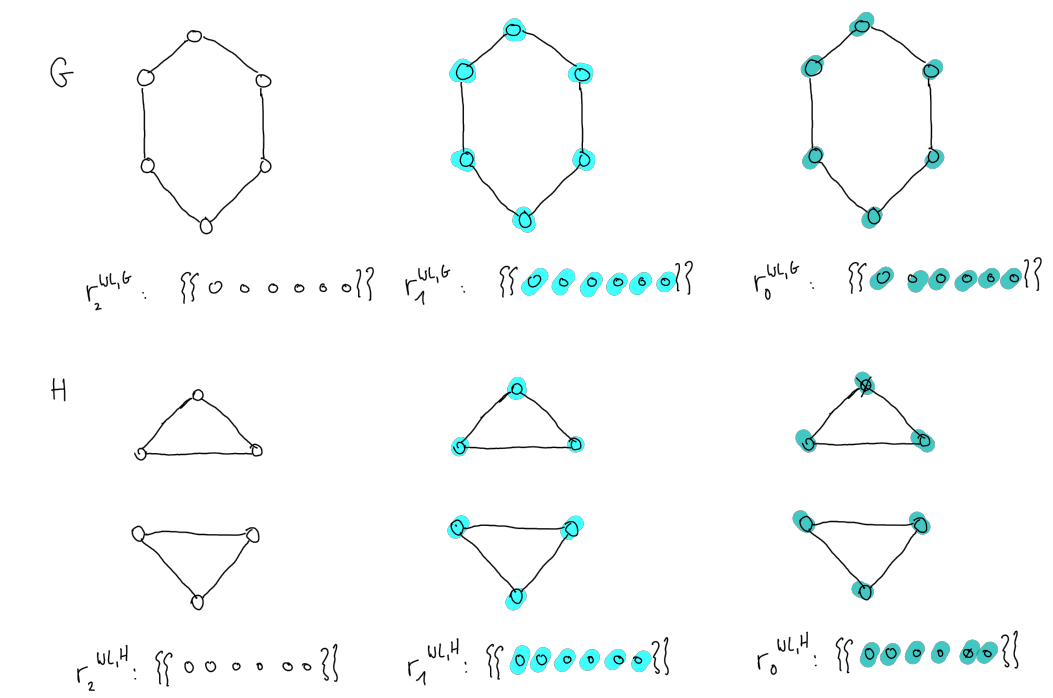
\includegraphics[width=0.7\linewidth]{images/nonisoGraphExampleWithIdWL}
	\caption{Example of non-isomorphic graphs with identical label histograms.}
	\label{fig:nonisographexamplewithidwl} %TODO: write LaTex
\end{figure}

This result allows us to test if two graphs $G$ and $H$ are not isomorphic. Therefore simply compute the multisets $\mset{ r_k^{\text{WL}, G}(v)| \ v\in V(G)}$ and $\mset{ r_k^{\text{WL}, H}(v)| \ v\in V(H)}$. If these multisets differ for any $0\le k\le \max\big( |V(G)|, \ |V(H)| \big)$ the graphs $G$ and $H$ are not isomorphic.

Note that if the two multisets are identical, the graphs might be isomorphic or not!

\subsubsection{Efficient computation of the WL labels}

Recall the Weisfeiler Lehman labeling scheme presented in equation \ref{eq:WLLabellingScheme}:
\[ r_{k+1}^{\text{WL}}(v) = \#_k \Big( r_k^{\text{WL}}(v), \ \text{id}_k\big( \mset{ r_k^{\text{WL}}(w)|\ w\in N(v)} \big) \Big) \]

To compute it efficiently, we need a fast way to hash multisets $X$ from $\mathcal{X}$. Let $<$ be a total order on $\mathcal{X}$, then sorting all elements in $X$ according to $<$ returns a unique results. Thus we can compute a canonical string of symbols for each multiset. This would already be a perfect hash function.

With a canonical string of a neighbor label multiset, we can now build a lookup table (on the fly) that assigns each pair (central vertex label and canonical string of neighbor labels) a unique (integer) id. 

%%%%%%%%%%%%%%%%%%%%%%%%%%%%%%%%%%
%%%%% Lecture 04 - 15.11.2021 %%%%
%%%%%%%%%%%%%%%%%%%%%%%%%%%%%%%%%%

\subsection{Message passing on GNNs}

We would like to train a GNN to implement the message passing, i.a. compute the update and aggregation function, which we have seen already in equation \ref{eq:MessagePassing}
\[ r_{k+1}(v) = \operatorname{upd}_k\Big(r_k (v), \operatorname{agg}_k\big( r_k(w)|\ w\in N(v) \big) \Big) \]

In its oldest form, a GNN layer is defined for all $v\in V(G)$ as
\begin{equation}\label{eq:GNNMessagePassing}
	r_{k+1}(v) = \sigma\Big( W_k^{\text{self}} r_k(v) \;+\; W_k^{\text{neigh}} \sum_{w\in N(v)} r_k(w) + b_k \Big)
\end{equation}
where\begin{itemize}
	\item $W_k^{\text{self}}, W_k^{\text{neigh}}\in \IR^{d_k\times d_{k+1}}$ are trainable parameter matrices, 
	\item $\sigma:\IR^{d_k+1}\to\IR^{d_k+1}$ is an element-wise non-linear function\\ (e.g. $\tanh$, ReLU or sigmoid) and 
	\item $b\in\IR^{d_{k+1}}$ denotes trainable bias parameters\cite{scarselli2008graph}.
\end{itemize} 

For now, lets assume that the weights and biases are chose appropriately and focus on the forward pass.

Let use $\theta_k$ to denote \textit{trainable weights in iteration} $k$ of the GNN. We will interpret this as a flattened vector, i.e. $\theta_k \in \IR^{2d_k d_{k+1} + d_{k+1}}$. 

Lets identify the update and aggregator function. The latter is trivial (and ensures permutation invariance):
\begin{itemize}
	\item[] $\operatorname{agg}_k \big( \mset{r_k(w)| \ w\in N(v)} \big) = \ \sum\limits_{w\in N(v)} r_k(v)$	
	\item[] $\operatorname{upd}_k = W^{\text{self}}_k r_k(v) + W^{\text{neigh}}_k \operatorname{agg}_k (\cdot) + b_{k+1}$
\end{itemize}

\paragraph{Example - Message Passing on a GNN}

Lets compute the next two representations for this example graph with a simple GNN:

\begin{figure}[H]
	\centering
	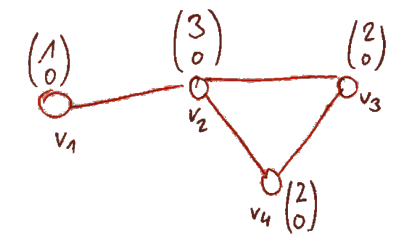
\includegraphics[width=0.7\linewidth]{images/exampleMessagePassingGNN}
	\caption{}
	\label{fig:examplemessagepassinggnn}
\end{figure} %TODO: Node labelling



\begin{minipage}{\textwidth}
	\begin{figure}[H]
		\centering
		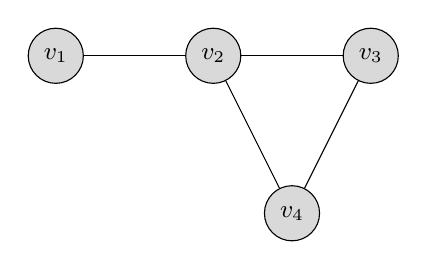
\begin{tikzpicture}[x=2cm,y=2cm] 
		\begin{scope}[scale=1]
		
		\tikzstyle{mycircle}=[circle,
		draw=black,
		fill=gray,
		fill opacity = 0.3,
		text opacity=1,
		inner sep=0pt,
		minimum size=7mm,
		font=\small
		]
		
		\coordinate (px1) at (0, 1);		
		\coordinate (px2) at (1, 1);
		\coordinate (px3) at (2, 1);
		\coordinate (px4) at (1.5, 0);
		
		
		\node[mycircle] (x1) at (px1) {$v_1$};	
		\node[mycircle] (x2) at (px2) {$v_2$};
		\node[mycircle] (x3) at (px3) {$v_3$};	
		\node[mycircle] (x4) at (px4) {$v_4$};
		
		\draw[-] (x1) -- (x2);
		\draw[-] (x2) -- (x3);
		\draw[-] (x3) -- (x4);
		\draw[-] (x2) -- (x4);
		
		
		\end{scope}
		\end{tikzpicture}
	\end{figure}
	\captionof{figure}{Example for the closeness centrality measure}
	\label{fig:closenesscentrality3}
\end{minipage}

Initialize the GNN with 
\begin{multicols}{2} \begin{itemize}
	\item $\sigma = \text{id}$
	\item $b_i = \begin{bmatrix} 0 \\ 0 \end{bmatrix}$
	\item $W_i^{\text{self}} \ \ \ = \begin{bmatrix} 1 & 1 \\ 0 & 1\end{bmatrix}$
	\item $W_i^{\text{neigh}} = \begin{bmatrix} 1 & 1 \\ 1 & 0\end{bmatrix}$	
\end{itemize}\end{multicols}
We compute:
\begin{flalign*}
	r_1(v_1) &= W_0^{\text{self}}r_0(v_1) + W_0^{\text{neigh}}\Big( r_0(v_2) \Big) + b_i\\
	&= \begin{bmatrix} 1 & 1 \\ 0 & 1\end{bmatrix} \begin{bmatrix} 1 \\ 0 \end{bmatrix} +
	\begin{bmatrix} 1 & 1 \\ 1 & 0\end{bmatrix} \begin{bmatrix} 3 \\ 0 \end{bmatrix} + \begin{bmatrix} 0 \\ 0 \end{bmatrix}\\
	&= \begin{bmatrix} 1 \\ 0 \end{bmatrix} + \begin{bmatrix} 3 \\ 3 \end{bmatrix} + \begin{bmatrix} 0 \\ 0 \end{bmatrix}
	&= \begin{bmatrix} 4 \\ 3 \end{bmatrix}\\	
	r_1(v_2) &= W_0^{\text{self}}r_0(v_2) + W_0^{\text{neigh}}\Big( r_0(v_1) + r_0(v_3) + r_0(v_4) \Big) + b_i\\
	&= \begin{bmatrix} 1 & 1 \\ 0 & 1\end{bmatrix} \begin{bmatrix} 3 \\ 0 \end{bmatrix} +
	\begin{bmatrix} 1 & 1 \\ 1 & 0\end{bmatrix} \Big(\begin{bmatrix} 1 \\ 0 \end{bmatrix} + \begin{bmatrix} 2 \\ 0 \end{bmatrix} + \begin{bmatrix} 2 \\ 0 \end{bmatrix} \Big) + \begin{bmatrix} 0 \\ 0 \end{bmatrix}\\
	&= \begin{bmatrix} 3 \\ 0 \end{bmatrix} + \begin{bmatrix} 5 \\ 5 \end{bmatrix} + \begin{bmatrix} 0 \\ 0 \end{bmatrix}
	&= \begin{bmatrix} 8 \\ 5 \end{bmatrix}\\
	r_1(v_3) &= W_0^{\text{self}}r_0(v_3) + W_0^{\text{neigh}}\Big( r_0(v_2) + r_0(v_4) \Big) + b_i\\
	&= \begin{bmatrix} 1 & 1 \\ 0 & 1\end{bmatrix} \begin{bmatrix} 2 \\ 0 \end{bmatrix} +
	\begin{bmatrix} 1 & 1 \\ 1 & 0\end{bmatrix} \Big(\begin{bmatrix} 3 \\ 0 \end{bmatrix} + \begin{bmatrix} 2 \\ 0 \end{bmatrix} \Big) + \begin{bmatrix} 0 \\ 0 \end{bmatrix}\\
	&= \begin{bmatrix} 2 \\ 0 \end{bmatrix} + \begin{bmatrix} 5 \\ 5 \end{bmatrix} + \begin{bmatrix} 0 \\ 0 \end{bmatrix}
	&= \begin{bmatrix} 7 \\ 5 \end{bmatrix}\\
	r_1(v_4) &= r_1(v_3) &= \begin{bmatrix} 7 \\ 5 \end{bmatrix}
\end{flalign*}
For the next iteration it is analogously:
\begin{flalign*}
	r_2(v_1) &= \begin{bmatrix} 1 & 1 \\ 0 & 1\end{bmatrix} \begin{bmatrix} 4 \\ 3 \end{bmatrix} +
	\begin{bmatrix} 1 & 1 \\ 1 & 0\end{bmatrix} \Big( \begin{bmatrix} 8 \\ 5 \end{bmatrix}\Big) + \begin{bmatrix} 0 \\ 0 \end{bmatrix}\\
	&= \begin{bmatrix} 7 \\ 3 \end{bmatrix} + \begin{bmatrix} 13 \\ 8 \end{bmatrix} + \begin{bmatrix} 0 \\ 0 \end{bmatrix}
	&= \begin{bmatrix} 20 \\ 11 \end{bmatrix}\\	
	r_2(v_2) &= \begin{bmatrix} 1 & 1 \\ 0 & 1\end{bmatrix} \begin{bmatrix} 8 \\ 5 \end{bmatrix} +
	\begin{bmatrix} 1 & 1 \\ 1 & 0\end{bmatrix} \Big(\begin{bmatrix} 4 \\ 3 \end{bmatrix} + \begin{bmatrix} 7 \\ 5 \end{bmatrix} + \begin{bmatrix} 7 \\ 5 \end{bmatrix} \Big) + \begin{bmatrix} 0 \\ 0 \end{bmatrix}\\
	&= \begin{bmatrix} 13 \\ 5 \end{bmatrix} + \begin{bmatrix} 31 \\ 18 \end{bmatrix} + \begin{bmatrix} 0 \\ 0 \end{bmatrix}
	&= \begin{bmatrix} 44 \\ 23 \end{bmatrix}\\
	r_2(v_3) &= \begin{bmatrix} 1 & 1 \\ 0 & 1\end{bmatrix} \begin{bmatrix} 7 \\ 5 \end{bmatrix} +
	\begin{bmatrix} 1 & 1 \\ 1 & 0\end{bmatrix} \Big(\begin{bmatrix} 7 \\ 5 \end{bmatrix} + \begin{bmatrix} 8 \\ 5 \end{bmatrix} \Big) + \begin{bmatrix} 0 \\ 0 \end{bmatrix}\\
	&= \begin{bmatrix} 12 \\ 5 \end{bmatrix} + \begin{bmatrix} 25 \\ 15 \end{bmatrix} + \begin{bmatrix} 0 \\ 0 \end{bmatrix}
	&= \begin{bmatrix} 37 \\ 20 \end{bmatrix}\\
	r_2(v_4) &= r_2(v_3) &= \begin{bmatrix} 37 \\ 20 \end{bmatrix}
\end{flalign*}

Note that the numbers in this example tend to grow large rather quickly. In particular, one might expect, that the representations of high degree vertices will contain large values, with a large difference to the values of representations of low degree vertices.

This might lead to numerical instabilities and difficulties in optimization of the loss function.

To prevent this one may swap the sum aggregator with the \textit{mean aggregator}. This also limits the influence of individual vertices in the training.

Another variation is to use the \textit{symmetric normalization} aggregator:

\[ \operatorname{agg}_k(\cdot) = \sum_{w\in N(v)} \frac{ r_k(w) }{ \sqrt{ |N(v)|\ |N(w)| } } \]

\subsection{Message passing on GCNs}

A very popular variant of GNNs are \textbf{Graph Convolutional Neural Networks} (\textbf{GCNs})\cite{kipf2016semi}. These use symmetric normalization and do not distinguish between representations of a vertex $v$ and its neighbors $w\in N(v)$. Thus by construction, they are likely to lose information:
\begin{equation}\label{eq:GCNUpdate}
	r_{k+1} (v)= \text{ReLU}\Big( W_k\ \sum_{w\in N(G)\cup\{v\}} \frac{r_k(w)}{ \sqrt{|N(v)|\ |N(w)|}} +b_k  \Big)
\end{equation}
Again, $W\in \IR^{d_k \times d_{k+1}}$ and $b_k\in \IR^{d_{k+1}}$ are trainable parameters.

Note that symmetric normalization (partially) inhibits to learn from the degree of a vertex.
 

\subsection{Message passing on GINs}

Another variant adds a multiple layer trainable Neural Network in each message passing step. These are called \textbf{Graph Isomorphism Networks} (\textbf{GINs})\cite{xu2018powerful}. Let $NN_{\theta_k}$ be a (multilayer) Neural Network (with trainable weights and element-wise non-linearities). Let $\epsilon_k\in \IR$ be a trainable weights. Then the update step of a GINs, using these parameters, can be described as:

\begin{equation}\label{eq:GINUpdate}
	r_{k+1}(v) = \operatorname{NN}_{\theta_k} \Big( (1+\epsilon_k) r_k(v) + \ \sum_{w\in N(v)} r_k(w)+ b_k \Big)
\end{equation}

There are a lot of freedoms when configuring GINs. Common hyper-parameters that can be learned are:\begin{itemize}
	\item The number of layers in the MLP (often only one or two hidden layers).
	\item The number of units per hidden layer (often 16 or 32 units).
	\item The non-linearity function (often ReLU).
\end{itemize}

\subsection{Training GNNs}

\subsubsection{Training GNNs for vertex classification}

Assume that we are in a supervised vertex classification setting. Thus for each vertex $v\in V(G)$ we want to predict a discrete class $y(v)\in C$ for some finite set of classes $C=\{c_1,\dots, c_d\}$.

We are given a finite set of vertices $V\subseteq V(G)$ with known labels $\{ y(v)|\ v\in V \}$.

As usual we can use (stochastic) gradient descent, backpropagation and a differentiable loss function to train a suitable GNN. Neural Networks for classification tasks are often trained with the \textbf{negative log likelihood} loss functions of a \textbf{softmax classification}:
\begin{equation}\label{eq:NegLogLikelihoodSoftmax}
	L_{G,y}(h_\theta) = \sum_{v\in V} -\log\Big( \trn{\vv{y}(v)} \softmax\big(r(v)\big) \Big)
\end{equation}
where $\vv{y}(v) \in \one^d$ is a \textit{one-hot vector} encoding the class of $v$. That is for $y(v)=c_i$ have the $i$-th unit vector as the one-hot encoding $\vv{y}(v)=e_i$. $r(v)\in \IR^d$ is the (last hidden) representation of $v$.

\begin{Definition}[Softmax function]{def:Softmax}
	The \textbf{softmax function}
	\[ \softmax( x )_i = \frac{\exp(x_i)}{\sum_{j=1}^{d}\exp(x_j)} \]
	maps a $d$-dimensional vector $x\in\IR^d$ to a $d$-dimensional vector $\hat{y}$ with 
	\[ \sum_{j=1}^{d} \hat{y}_i = 1 \]
	Hence, the entries of the output $\hat{y}$ can be interpreted as probabilities to belong to a certain class of $d$ classes.
	
	In most cases, the dimension with the largest entry will be mapped to a value close to one - and the rest respectively close to zero (hence the name).
\end{Definition}

Recall that message passing Neural Networks compute some representation $r_k(v)\in \IR^d{d_k}$ for some $d_k$ - that is one representation for all $k$ iterations over all $d$ possible representation values. $d_k$ usually depends on the dimensionality of the input representation $r_0 :V(G) \to \IR^{d_0}$ and $d_k$ is not equal to the number of classes in the vertex classification problem $d=|C|$.

Hence, we have to transform the message passing representations to representations that are suitable as input to the softmax function. To do this, we can use another Neural Network $NN_{\theta^\prime}:\IR^{d_k}\to\IR^d$ (with learnable parameters $\theta^\prime$). Then we can minimize the loss function

\begin{equation}
	L_{G,y}(h_{k, \theta, \theta^\prime}) = \sum_{v\in V} -\log\Big( \trn{\vv{y}(v)} \softmax\big( \operatorname{NN}_{\theta^\prime}(r(v))\big) \Big)
\end{equation}

Lets take a closer look at the parameters. It is:
\[ v \stackrel{\text{given}}{\mapsto} r_0(v) \stackrel{\operatorname{upd}_{\theta_0}}{\mapsto} r_1(v) \stackrel{\operatorname{upd}_{\theta_1}}{\mapsto} \dots \stackrel{\operatorname{upd}_{\theta_{k-1}}}{\mapsto} r_k(v) \stackrel{\operatorname{NN}_{\theta^\prime}}{\mapsto} x(v) \stackrel{\softmax}{\mapsto} \hat{y}(v)  \]

Since all functions between the representations $r_0(v)$ and $\hat{y}(v)$ are differentiable with respect to the parameters $\theta_0 , \dots, \theta_{k-1}, \theta^\prime$ ne can use the chain rule to automatically compute the gradient with respect to them:

\begin{equation}\label{eq:NablaNegLogLikelihoodSoftmax}
	\nabla L_{G,y}(h_{k,\theta_0,\dots,\theta_{k-1}, \theta^\prime}) = \nabla\Big( -\log \circ \softmax \circ \operatorname{NN}_{\theta^\prime} \circ \operatorname{upd}_{\theta_{k-1}} \circ \dots \circ \operatorname{upd}_{\theta_{0}}  \Big)
\end{equation}

The weights are updated according to some chosen strategy.

\begin{algorithm}[H]
	\caption{GNN - Vertex representation - ONE EPOCH} \label{alg:GNNVertexRep} 
	\begin{tabbing}
		\textbf{Output:} \= \kill
		\textbf{Input:} \>a training set $V\subseteq V(G)$ with known classes $y:V\to C$,\\
		\>learning rage $\gamma$,\\
		\>a Neural Network to learn the vertex representation, given a softmax $\operatorname{NN}_{\theta^\prime}$,\\
		\>number of message passing steps $k$ and\\
		\>the initial vertex representation $r_0(v)$ for all vertices $v\in V(G)$.\\
		\textbf{Output:} \>updated weights $\theta_0, \dots, \theta_{k-1}, \theta^\prime$.
	\end{tabbing}	
	\begin{algorithmic}[1]		
		\State Run $k$ iterations of the GNN message passing for all  $v\in  V(G)$
		\State Apply $\operatorname{NN}_{\theta^\prime}$ to the resulting representations $r_k(v)$ for all $v\in V(G)$
		\State Compute $L_{G,y}(h_{k, \theta_0, \dots, \theta_{k-1}, \theta^\prime})$
		\State Update the weights by setting
		\[ (\theta_0, \dots, \theta_{k-1}, \theta^\prime) \ = \ (\theta_0, \dots, \theta_{k-1}, \theta^\prime) - \gamma \nabla L_{G, y}(h_{k,\theta_0, \dots, \theta_{k-1}, \theta^\prime}) \]
	\end{algorithmic}
	Note that this algorithm processes the whole training dataset at once (i.e. with gradient descent).
\end{algorithm}

Usually NNs are trained one mini-batch at a time (i.e. with stochastic gradient descent). To apply this to the GNN, we need to compute a (intermediate) representation for additional vertices (outside of the mini-batch).

\begin{algorithm}[H]
	\caption{GNN - Vertex representation - ONE EPOCH - Mini-batch} \label{alg:GNNVertexRepMiniBatch} 
	\begin{tabbing}
		\textbf{Output:} \= \kill
		\textbf{Input:} \>a training \textbf{batch} $B\subseteq V\subseteq V(G)$ with known classes $y:V\to C$,\\
		\>learning rage $\gamma$,\\
		\>a Neural Network to learn the vertex representation, given a softmax $\operatorname{NN}_{\theta^\prime}$,\\
		\>number of message passing steps $k$ and\\
		\>the initial vertex representation $r_0(v)$ for all vertices $v\in V(G)$.\\
		\textbf{Output:} \>updated weights $\theta_0, \dots, \theta_{k-1}, \theta^\prime$.
	\end{tabbing}	
	\begin{algorithmic}[1]		
		\For{$i = 1,\dots, k$}
			\State Compute the $i$-hop neighborhoods $N_i(v)$ for all $v\in B$
		\EndFor
		\For{$i = 1,\dots, k$}
			\State Compute $r_i(w)$ for all $w\in N_{k-i}(v)$ for all $v\in B$
		\EndFor
		\State Apply $\operatorname{NN}_{\theta^\prime}$ to the resulting representations $r_k(v)$ for all $v\in B$
		\State Compute $L_{G,y}(h_{k, \theta_0, \dots, \theta_{k-1}, \theta^\prime})$
		\State Update the weights by setting
		\[ (\theta_0, \dots, \theta_{k-1}, \theta^\prime) \ = \ (\theta_0, \dots, \theta_{k-1}, \theta^\prime) - \gamma \nabla L_{G, y}(h_{k,\theta_0, \dots, \theta_{k-1}, \theta^\prime}) \]
	\end{algorithmic}
	Note that this algorithm processes the whole training dataset at once (i.e. with gradient descent).
\end{algorithm}

Often, \textbf{weight sharing} is applied between GNN iterations. That is, we use the same functions $\operatorname{upd}$ and $\operatorname{agg}$ for each iteration $k$ of the message passing framework. This means that we set $\theta_0 = \theta_1 = \dots = \theta_{k-1}$ and update these hyper-parameters simultaneously from the different iterations during backpropagation. This can be beneficial but also a drawback for learning.

One may ask, if these algorithms \ref{alg:GNNVertexRep} and \ref{alg:GNNVertexRepMiniBatch} follow the principle of \textit{supervised learning}.

\begin{Definition}[Supervised learning]{def:SupervisedLearning}
	The \textbf{supervised learning} principle is fulfilled, it the learning algorithm works based on the following in- and outputs:
	\begin{tabbing}
		\textbf{Output:} \= \kill
		\textbf{Input:} \>a domain set $\mathcal{X}$,\\
		\>a target domain set $\mathcal{Y}$,\\
		\>a \textit{hypothesis class} $\mathcal{H}\subseteq \{ h|\ h:\mathcal{X}\to \mathcal{Y} \}$,\\
		\>a finite set $X\subseteq \mathcal{X}$ and known target values $y(x)$ for all $x\in X$ and\\
		\>a loss function $L_y:\mathcal{H}\to \IR$.\\		
		\textbf{Output:} \>$\amin{h\in \mathcal{H}} L_y(h)$.
	\end{tabbing}
\end{Definition}

Now lets apply this to the vertex representation learning task. We have:

\begin{tabbing}
	\textbf{Output:} \= \kill
	\textbf{Input:} \>a graph $G$ with labeling functions $f_V$ and $f_E$,\\
	\>a \textit{hypothesis class} $\mathcal{H}\subseteq \{ h|\ h: V(G)\to \mathcal{Y} \}$,\\
	\>a finite set $V^\prime\subseteq V(G)$ and known target values $y(v)$ for all $v\in V^\prime$ and\\
	\>a loss function $L_{G, y}:\mathcal{H}\to \IR$.\\
%	\textbf{Output:} \>$\amin{h\in \mathcal{H}} L_y(h)$.
\end{tabbing}

Now consider the aggregation step in the message passing framework (\ref{eq:MessagePassing})
\[ 
r_{k+1}(v) = \operatorname{upd}_k \Big( r_k(v), \operatorname{agg}_k \big(r_k(w)|\ w\in N(v)\big) \Big)
\]
What happens when $w\in N(v)$ is not part of $V^\prime$? The update operation requires information from objects that are \textit{not} part of the training set in order to construct the (novel) vertex representations.
On top of that, it is likely information from an object in the test or validation set. Thus actually, we require the full graph $G$ as input to our training. We cannot (by assumption) learn functions over vertices that were not part of $V(G)$ at the time of training. This is called \textbf{transductive learning} or \textbf{transductive inference}.
We are trying to predict a target feature for a specifically known finite set of possible test instances $V(G)\backslash V^\prime$.

%%%%%%%%%%%%%%%%%%%%%%%%%%%%%%%%%%
%%%%% Lecture 05 - 22.11.2021 %%%%
%%%%%%%%%%%%%%%%%%%%%%%%%%%%%%%%%%

\chapter{Transactional Graph Learning} %Learning graph representations for graph classes

Up to now, we have tried to represent and learn from vertices in a single graph. In this chapter, we will consider learning functions over whole graphs. Since the term Graph Learning is overloaded with meaning, we will call this task \textbf{Transactional Graph Learning}. We will call individual graphs (\textbf{graph}) \textbf{transactions}. The objective of Transactional Graph Learning is to determine whether a graph belongs to a \textbf{graph class}, which is a (typically finite) set of graphs, or not.

Examples of graph classes are:\begin{itemize}
	\item Graphs
	\item Forests (cycle free graphs)
	\item Trees (connected and cycle free graphs)
	\item Molecular graphs\\
	(Graphs  that describe the structural formulas of valid molecules.)
	\item 
\end{itemize}

Similar to definition \ref{def:GraphAttributesLabels} lets define additional data on graphs, their vertices and edges for a whole graph class.

\begin{Definition}[Graph class attributes and labels] {def:GraphClassAttributesLabels}
	Given a graph class $\mathcal{G}$ containing transactions (graphs).
	The vertices and edges in these transactions may be labeled (or attributed).
	
	We formalize this using appropriate \textbf{feature spaces} $\mathcal{X}$, $\mathcal{X}^\prime$ and $\mathcal{X}^{\prime\prime}$:
	\[ f_G: \mathcal{G} \to \mathcal{X},\qquad\qquad f_V: \bigcup_{G \in\mathcal{G}} V(G) \to \mathcal{X}^\prime,\qquad\qquad f_E:\bigcup_{G \in\mathcal{G}} E(G) \to \mathcal{X}^{\prime \prime}\]	
\end{Definition}


%TODO: Does the union here imply a countable set? If so, note that countability is not necessary!

Note that in one learning task, we assume that all graphs in a graph class are labeled with values from the same feature spaces and these values are meaningfully comparable.

\begin{Definition}[Transactional Graph Learning]{def:transactionalGraphLearning}
	\begin{tabbing}
		\textbf{Output:} \= \kill
		\textbf{Input:} \>a class of graphs $\mathcal{G}$,\\
		\>a target domain set $\mathcal{Y}$,\\
		\>a \textit{hypothesis class} $\mathcal{H}\subseteq \{ h|\ h:\mathcal{G}\to \mathcal{Y} \}$,\\
		\>a finite set $D\subseteq \mathcal{G}$ and known target values $y(G)$ for all $G\in D$ and\\
		\>a loss function $L_y:\mathcal{H}\to \IR$.\\		
		\textbf{Output:} \>$\amin{h\in \mathcal{H}} L_y(h)$.
	\end{tabbing}
	Note that in Transactional Graph Learning one usually assumes that \textbf{isomorphic graphs behave identically}.
\end{Definition}

\section{Multiset graph representations}

In order to use standard machine learning algorithms, we are in need of a vector representation for graphs $r:\mathcal{G}\to\IR^d$. The main idea is to use the vertex representations that are discussed in the previous chapter the represent a whole graph $G$.

A trivial example is the list of all occurring vertex degrees:
\[ \vec{r}(G) := \bigoplus_{v\in V(G)} r(v)\qquad \in \IR^{d|V(G)|} \]
Of course this is permutation sensitive. One may get around this by using multisets or sorted lists of vertex degrees. More challenging is the concern, that graphs can have different amounts of vertices. Hence this representation for $r_G \in \IR^{d|V(G)|}$ and $r_H \in \IR^{d|V(H)|}$ cannot be used to define a function $r:\mathcal{G}\to\IR^{d^\prime}$ with fixed $d^{\prime}$.

Thus in general it is better to use a common feature space $\mathcal{X}$ and define the graph representation $r_{\text{MS}}$ as invariant multisets. We will use some vertex representation (e.g. vertex degree) $r:V(G) \to \mathcal{X}$ and set:
\begin{equation}\label{eq:MultisetGraphRepresentation}
	r_{\text{MS}}(G) = \mset{ r(v)|\ v\in V(G) }\qquad\in \IN^{|\mathcal{X}|}
\end{equation}

Note that $\mathcal{X}$ can have a practically infeasible number of elements (possibly infinitely many). Thus such \textbf{multiset graph representations} are useful for \textit{discrete} vertex representations. For example vertex degrees, vertex degeneracies, triangle counts, other individual graphlet counts or Weisfeiler-Lehman vertex labels.

For all these examples, the multiset representation can be used for \textit{overlap based similarities}.

We can represent multisets as vectors with one dimension per element of $\mathcal{X}$ that stores a count. When dealing with finite transactional graph databases, we know that
\[ |\mset{r(v)|\ v\in V(G) }| = |V(G)| \]
That means that there are always only finitely many entries that are nonzero for each graph $G\in\mathcal{G}$. That means we can use \textbf{sparse vectors} in practice to efficiently store the multiset representation $r_{\text{MS}}(G) \in \IN^{|\mathcal{X}|}$ in our finite memory, even if $|\mathcal{X}| = \infty$.

\begin{Theorem}[Multiset graph representation respects isomorphism] {thm:MSGraphRepIso}
	Let $G, H\in\mathcal{G}$ be two graphs and $\varphi:V(G)\to V(H)$ an isomorphism that respects their vertex features $f_V : \bigcup_{G\in \mathcal{G}} V(G) \to \mathcal{X}^\prime$. Let $r_{\text{MS}}:\mathcal{G} \to \IN^{\mathcal{X}^{\prime}}$ be a multiset graph representation of these features: 
	\[ r_{\text{MS}}(G) = \mset{ f_V(v)|\ v\in V(G) } \]
	
	Then 
	\[ r_{\text{MS}}(G) = r_{\text{MS}}(H) \]
\end{Theorem}
\begin{Proof}
	Exercise. %TODO
\end{Proof}

We say the multiset graph representation is \textit{invariant under isomorphism}. They may or may not map non-isomorphic graphs to different values.

\subsection{Histogram graph representations}

Recall that we have earlier discussed \textit{histogram aggregators}. Let $\mathcal{X}$ be a set and $B_1,B_2,\dots, B_k\subseteq \mathcal{X}$ be bins. Then, for $X\in \IN^{\mathcal{X}}$ and $B_i$ we can define
\[ \operatorname{count}_{B_i}(X) = |\mset{ x\in X| \ x\in B_i }| \]
and a histogram as a mapping $\operatorname{hist}_{B_1,\dots,B_k}:\IN^{\mathcal{X}} \to \IN^k$ as
\[ \operatorname{hist}_{B_1,\dots, B_k}(X) = \big( \operatorname{count}_{B_1}(X),\dots, \operatorname{count}_{B_k}(X) \big) \]

Note that histograms generalize multisets in the sense that \textit{a multiset is a histogram where each bin contains a single object}. One can define a histogram aggregator that counts the occurrences of each individual object in (finite or countably infinite) $\mathcal{X}$. One can also define weighted versions where one sums over the weights of objects in a bin.

Histograms can be seen as discrete distributions. During their definition one can influence the dimensionality of the resulting graph representation.

\begin{Theorem}[Histogram graph representation respects multiset graph representations] {thm:MSGraphRepMSGraphRep}
	Let $G, H\in\mathcal{G}$ be two graphs and $\varphi:V(G)\to V(H)$ an isomorphism that respects their vertex features $f_V : \bigcup_{G\in \mathcal{G}} V(G) \to \mathcal{X}^\prime$. Let $r_{\text{MS}}:\mathcal{G} \to \IN^{\mathcal{X}^{\prime}}$ be a multiset graph representation of these features: 
	\[ r_{\text{MS}}(G) = \mset{ f_V(v)|\ v\in V(G) } \]
	Let $\operatorname{hist}_{B_1,\dots, B_k}:\IN^{\mathcal{X}^\prime}\to\IN^{k}$ be a histogram representation:
	\[ \operatorname{hist}_{B_1,\dots, B_k}(X) = \big( \operatorname{count}_{B_1}(X),\dots, \operatorname{count}_{B_k}(X) \big) \]
	
	Then 
	\[ \operatorname{hist}_{B_1,\dots, B_k}\big(r_{\text{MS}}(G)\big) = \operatorname{hist}_{B_1,\dots, B_k}\big(r_{\text{MS}}(H)\big) \]
\end{Theorem}
\begin{Proof}
	From theorem \ref{thm:MSGraphRepIso}, we know that the multiset representations of isomorphic graphs are identical. Since $\operatorname{hist}_{B_1,\dots, B_k}$ is a function, we know that it hence must map the identical images of $G$ and $H$ to the same value:
	\[ r_{\text{MS}}(G) = r_{\text{MS}}(H) \]
\end{Proof}

Note that isomorphism respects the original labeling. Hence, graphs with different original label multisets can never be isomorphic. One may need to take extra care with respect to original labels in order to not have the representation denote an isomorphism where there is no one to be found.

\begin{minipage}{\textwidth}
	\begin{minipage}{0.5\textwidth}\begin{figure}[H]
		\centering
		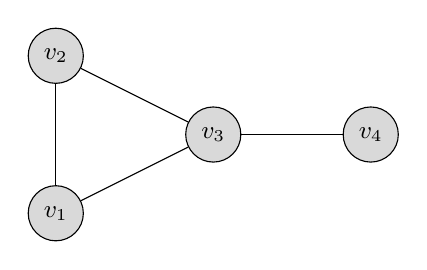
\begin{tikzpicture}[x=2cm,y=2cm] 
		\begin{scope}[scale=1]
		
		\tikzstyle{mycircle}=[circle,
		draw=black,
		fill=gray,
		fill opacity = 0.3,
		text opacity=1,
		inner sep=0pt,
		minimum size=7mm,
		font=\small
		]
		
		\coordinate (px1) at (0, 0);		
		\coordinate (px2) at (0, 1);
		\coordinate (px3) at (1, 0.5);
		\coordinate (px4) at (2, 0.5);
		
		
		\node[mycircle] (x1) at (px1) {$v_1$};	
		\node[mycircle] (x2) at (px2) {$v_2$};
		\node[mycircle] (x3) at (px3) {$v_3$};	
		\node[mycircle] (x4) at (px4) {$v_4$};
		
		\draw[-] (x1) -- (x2);
		\draw[-] (x2) -- (x3);
		\draw[-] (x3) -- (x4);
		\draw[-] (x3) -- (x1);
		
		
		\end{scope}
		\end{tikzpicture}
	\end{figure}	
	\end{minipage}
	\begin{minipage}{0.5\textwidth}\begin{tabular}{l || c | c | c | c || r}
		& $v_1$ & $v_2$ & $v_3$ & $v_4$ & $\sum$ \\ \hline
		edge & $2$ & $3$ & $2$ & $1$ & $8$\\
		$3$-path & $1$ & $2$ & $1$ & $2$ & $6$ \\
		triangle & $1$ & $1$ & $1$ & $0$ & $3$ \\
	\end{tabular}
	\captionof{table}{Exapmle: Graphlet counting (of induced subgraphs).}
	\end{minipage}
\end{minipage}

\section{GNNs for Transactional Graph Learning}

Given a set of graphs for training, we can extend our neural network from
computing vertex representations to graph representations. After a fixed number of message passing layers to compute vertex representations,we add a final aggregator layer that aggregates all vertex representations in the graph.
Conceptually, for the last step we add a \enquote{hypervertex} that is connected to all vertices in the graph and aggregate over its neighbors and then update. The resulting \textbf{hypervertex representation} becomes the graph representation.

\begin{algorithm}[H]
	\caption{GNN - Transactional Graph Learning - ONE EPOCH} \label{alg:GNNTransactionalGraphLearning} 
	\begin{tabbing}
		\textbf{Output:} \= \kill
		\textbf{Input:} \>a training set $D \subseteq \mathcal{G}$ with known classes $y:D\to C$,\\
		\>learning rage $\gamma$,\\
		\>a Neural Network to learn the graph representation, given a softmax $\operatorname{NN}_{\theta^\prime}$,\\
		\>number of message passing steps $k$ and\\
		\>the initial vertex representation $r_0(v)$ for all vertices $v\in V(G)$.\\
		\textbf{Output:} \>updated weights $\theta_0, \dots, \theta_{k-1}, \theta_{\text{graph}}, \theta^\prime$.
	\end{tabbing}	
	\begin{algorithmic}[1]		
		\For{$G\in D$}
			\State Run $k$ iterations of your GNN message passing for all $v\in V(G)$
			\State Aggregate the vertex representations of all vertices in $G$
			\State Update the result to obtain a graph representation $r_{\text{graph}}(G)$
		\EndFor
		\State Apply $\operatorname{NN}_{\theta^\prime}$ to the resulting representations $r_{\text{graph}}(G)$ for all $G\in \mathcal{G}$
		\State Compute $L_{y}(h_{k, \theta_0, \dots, \theta_{k-1}, \theta_{\text{graph}}, \theta^\prime})$
		\State Update the weights by setting
		\[ (\theta_0, \dots, \theta_{k-1}, \theta^\prime) \ = \ (\theta_0, \dots, \theta_{k-1}, \theta_{\text{graph}}, \theta^\prime) - \gamma \nabla L_{G, y}(h_{k,\theta_0, \dots, \theta_{k-1}, \theta_{\text{graph}}, \theta^\prime}) \]
	\end{algorithmic}
\end{algorithm}

\section{Fast Forward Computation of Message Passing GNNs}

In the previous lectures (equation \ref{eq:GNNMessagePassing}), we have formulated the message passing framework on a per vertex basis. If we have to compute all vertex representations, anyway, we can reformulate the message passing NN using \textit{matrix vector operations} as follows:

\begin{equation}\label{eq:GNNMessagePassingFastForward}
	R_{k+1} = \sigma\Big( R_k W_k^{\text{self}} + A_G R_k R_k W_k^{\text{neigh}} + b_k \Big)
\end{equation}
Again $W_k^{\text{self}}, W_k^{\text{neigh}}\in\IR^{d_k \times d_{k+1}}$ and $b\in\IR^{d_{k+1}}$ are trainable weights (matrices). $A_G$ is a (sparse) adjacency matrix of $G$ and $R_k \in \IR^{|V(G)|\times d_k}$ is a row matrix of vertex representations.

%%%%%%%%%%%%%%%%%%%%%%%%%%%%%%%%%%
%%%%% Lecture 06 - 29.11.2021 %%%%
%%%%%%%%%%%%%%%%%%%%%%%%%%%%%%%%%%

\section{Complete representations}

Note that with theorem \ref{thm:MSGraphRepIso} we showed that the multiset graph representation is invariant under isomorphism, but may or may not map non-isomorphic graphs to different values. We now consider functions that map given graphs to different values \textit{if and only if} they are not isomorphic: 

\begin{Definition}[Complete representation of graph classes] {def:CompleteRepresentationFunction}
	Let $\mathcal{G}$ be a graph class and $\mathcal{Y}$ be some (feature) space. We call $c:\mathcal{G}\to\mathcal{Y}$ a \textbf{complete representation function of} $\mathcal{G}$ if
	\[ \forall G,H\in\mathcal{G}:\qquad c(G) = c(H) \ \iff\ G \text{ is isomorphic to } H \]
	and $c(G)=c(H)$ can be verified in \textit{polynomial time} in $\operatorname{size}\big( c(G) \big)$ and $\operatorname{size}\big( c(H) \big)$.
	
	Sometimes such functions are called \textbf{canonical functions} and their images are called \textbf{canonical strings} or \textbf{canonical labelings}.
\end{Definition}

Notice, that this property is a prerequisite to compute a (non-negative) distance between graphs. That is, if we cannot learn such functions, we will always have some objects that we cannot distinguish (by their image), although it might be necessary. 

Furthermore, isomorphism defines an equivalence relation on any graph class $\mathcal{G}$. We can consider the quotient space $\mathcal{G}_{\text{iso}}$ that contains exactly one representative graph $G_X$ for each subset $X\subseteq \mathcal{G}$ of pairwise isomorphic graphs in $\mathcal{G}$.

Let $f:\mathcal{G}\to\mathcal{Y}$ be invariant under isomorphism. Then this function induces a function $f_{\text{iso}}:\mathcal{G}_{\text{iso}}\to\mathcal{Y}$ with
\[ \forall X\subseteq \mathcal{G}:\qquad  f_{\text{iso}}(G_X)= f(G_X) \]

If $f$ is a complete representation on $\mathcal{G}$, then the induced $f_{\text{iso}}$ is \textit{injective} on $\mathcal{G}_{\text{iso}}$ (twp images are equal if and only if the inputs are equal).

\begin{Definition}[Expressiveness of functions] {def:ExpressivenessOfFunctions}
	Let $f,f^\prime:\mathcal{G}\to\mathcal{Y}$ be two functions that are invariant under isomorphism. $f^\prime$ is \textbf{less expressive} than $f$, denoted $f^\prime \le_{x} f$, if
	\[ f(G) = f(H) \ \implies \ f^\prime(G) = f^\prime(H) \]
	
	$f$ and $f^\prime$ are \textbf{equally expressive} if $f\le_{x} f^\prime$ and $f^\prime\le_{x} f$.
	
	$f^\prime$ is \textbf{strictly less expressive} than $f$ (written as $f^\prime <_{x} f$), if $f^\prime\le_{x} f$ and not $f\le_{x} f^\prime$.
\end{Definition}

\paragraph{Example of a complete representation} Let $\mathcal{G}$ be the class of all unlabeled graphs (i.e. $f_G, f_V, f_E$ are all constant). Let $<_{\text{Adj}}$ be a total order on the adjacency matrices. We assign any graph $G$ its \textit{smallest adjacency matrix among all permutations} of $V(G)$. Then two isomorphic graphs $G$, $H$ will be mapped to identical adjacency matrices.

More specifically, we can realize the total order on the adjacency matrices $<_{\text{Adj}}$ by \textit{lexicographical ordering} the flattened string representation of any adjacency matrix $G$.

While this function indeed is a complete representation, it cannot be computed efficiently (as far as we know). In fact, the naive algorithm for the representation on the previous slides iterates over all
permutations of the adjacency matrix and hence takes factorial time.

\begin{Theorem}[Complexity of complete representations] {thm:ComplexityOfCompleteRepresentations}
	Computing a complete representation for some graph class $\mathcal{G}$ is Isomorphism-hard.
	
	I.e. if we cannot decide if two graphs in $\mathcal{G}$ are isomorphic in polynomial time, then we cannot compute \textit{any} complete representation function for $\mathcal{G}$ in polynomial time.
\end{Theorem}
\begin{Proof}
	Suppose we can compute a complete representation $c:\mathcal{G} \to\mathcal{Y}$ for some suitable $\mathcal{Y}$ in polynomial time in $\operatorname{size}(G)$ for all $G\in\mathcal{G}$. Then we can, for two graphs $G,H\in\mathcal{G}$, compute $c(G)$ and $c(H)$ in polynomial time and evaluate $c(G)=c(H)$ in polynomial time.
	
	Hence, we have just found a polynomial time algorithm for checking isomorphism for graphs in $\mathcal{G}$.
\end{Proof}

We do not know the complexity of the isomorphism problem for the class of all graphs. Isomorphism \cite{babai2016graph} and recently computing a complete representation for the class of all graphs\cite{babai2019canonical} was shown to be solvable in \textbf{quasipolynomial time}.

Some more restricted graph classes have polynomial time complete representation functions. Various variants exists for trees\cite{chi2005frequent}, which allows to compute complete representations for forests, too. Also various graph classes allow for polynomial time algorithms, which in turn make it possible that a complete representation exists.


Note that this does not imply, that one cannot \textit{learn} a complete representation for the class of all graphs. Supervised learning from a fixed finite training dataset can be seen as \textit{constant time pre-processing}, i.e. it takes $\mathcal{O}(1)$ time. Thus, if we could learn a complete representation $c$ that is computable in polynomial time for any graph $G\in\mathcal{G}$, then this would imply a polynomial time algorithm for the isomorphism problem on $\mathcal{G}$.

GNNs promise to learn a suitable graph representation for any learning task. Thus lets explore if we can use them to learn complete representations for the class of all graphs.

Again, the Weisfeiler-Lehman vertex representations come to mind (definition \ref{def:WeisfeilerLehmanLabelPropagationScheme}). But we have the following result:

\begin{Theorem}[Incompleteness of Weisfeiler-Lehman representations] {thm:IncompletenessOfWL}
	Weisfeiler-Lehman representations are strictly less expressive on the class of all graphs than compete representations, i.e.
	\[ R_k^{\text{WL}} <_{x} c \]
	for any $k\in \IN$ and any complete representation $c$.
\end{Theorem}
\begin{Proof}
	There are a few counterexamples. These are non-isomorphic graphs with identical Weisfeiler-Lehman representations\cite{cai1992optimal}: %TODO: diesplay some of these graphs
\end{Proof}

\section{Expressive power of GNNs}

Before we present results about the expressiveness of GNNs, lets introduce a definition and a small theorem which we will use in the upcoming proofs:

\begin{Definition}[Strength of functions] {def:StrengthOrderOnFunctions}
	Let $f$ and $f^\prime$ be functions on some domain $\mathcal{X}$. We say $f^\prime$ is \textbf{less strong} than $f$ and write $f^\prime \tilde{\le} f$ if
	\[ \forall x,y\in \mathcal{X}:\qquad f(x) = f(y) \ \implies \ f^\prime(x) = f^\prime(y) \]
\end{Definition}

Note if $f$ and $f^\prime$ are functions on a graph class $\mathcal{G}$ such that $f$ and $f^\prime$ are invariant under isomorphism and $f^\prime \tilde{\le} f$, then $f^\prime$ is also less expressive than $f$, i.e. $f^\prime \le_{x} f$.

\begin{Theorem}[Obedience of weaker functions] {thm:ObedienceOfWeakerFunctions}
	Let $f^\prime$ and $f$ be two functions on some domain $\mathcal{X}$ and $f^\prime \tilde{\le} f$. Let $X,Y\subseteq \IN^{\mathcal{X}}$ be two multisets. Then
	\[ \Mset{f(x)|\ x\in X} = \Mset{f(x)|\ x\in Y} \ \implies \ \Mset{f^\prime(x)|\ x\in X} = \Mset{f^\prime(x)|\ x\in Y} \]
\end{Theorem}
\begin{Proof}
	The equality of two multisets $X^\prime, Y^\prime \subseteq \IN^{\mathcal{X}}$ means (by definition) that there exists a bijective function $b:X^\prime \to Y^\prime$ with $Y^\prime \ni b(x) = x\in X^\prime$.
	
	Thus the equality of multisets $\Mset{f(x)|\ x\in X} = \Mset{f(x)|\ x\in Y}$ implies that there is such a bijective function $b$ such that 
	\[ \forall x\in X:\qquad f(x) = b\big( f(x) \big) \]
	But we also have that $b\big( f(x) \big) = f(y)$ for some $y\in Y$ and hence $f(x)= f(y)$. So we also have a bijection $b^\prime:X\to Y$ such that $f(x) = f\big( b^\prime(x) \big)$.
	
	Now, by assumption $f(x) = f(y)$ implies $f^\prime(x) = f^\prime(y)$ and hence we have $f^\prime(x) = f^\prime\Big( b^\prime(x) \Big)$ for all $x\in X$ and hence also for all $f^\prime(x) \in \Mset{f^\prime(x)| x\in X}$.
\end{Proof}

\begin{Theorem}[GNNs are at most as expressive as Weisfeiler-Lehman representations\cite{xu2018powerful}] {thm:GNNAtMostExprAsWLRep}
	Let $\mathcal{G}$ be the class of all graphs and let $R_k:\mathcal{G}\to\IR^d$ be a representation of $\mathcal{G}$ computed by a message passing Graph Neural Network $r_k$ with $k$ iterations and some final graph aggregation step $\operatorname{agg}^\prime\Big( \mset{r_k(v)| \ v\in V(G)} \Big)$. Then
	\[ R_k \le_{x} R_k^{\text{WL}} \]
\end{Theorem}
\begin{Proof}
	The proof by induction has the following structure: We will show that for $R_k$ defined by $R_k(G)=\operatorname{agg}^\prime \big( \mset{r_k(v)|\ v\in V(G)} \big)$ with 
	\[ r_k(v) = \operatorname{upd}_k\Big( r_{k-1}(v), \ \operatorname{agg}_k\big( \mset{r_{k-1}| \ w\in N(v)} \big) \Big)\]
	for any choice of $\operatorname{agg}^\prime$, $\operatorname{agg}_k$ and $\operatorname{upd}_k$ it holds that
	\[ R_{k-1} \le_{x} R_{k-1}^{\text{WL}} \ \implies \ R_k\le_{x} R_k^{\text{WL}} \]
	That means if $R_{k-1}$ is less expressive than $R_{k-1}^{\text{WL}}$, then $R_k$ is less expressive than $R_k^{\text{WL}}$.
	
	We show this by showing that for 
	\[ r_k^{\text{WL}} = \# \Big( r_{k-1}^{\text{WL}}, \ \operatorname{id}\big( \mset{r_{k-1}(w)|\ w\in N(v)} \big) \Big) \]
	for any choice of $\operatorname{agg}_k$ and $\operatorname{upd}_k$ it holds that if
	\[ r_{k-1}^{\text{WL}}(v) = r_{k-1}^{\text{WL}}(u) \ \implies \ r_{k-1}(v) = r_{k-1}(u)\]
	then it is 
	\[ r_k^{\text{WL}}(v) = r_k^{\text{WL}}(u) \ \implies \ r_k(v) = r_k(u) \]
	
	
	\paragraph{Induction start}: Note that we are now talking about vertex representations and not about general $R$ functions defined over graphs. It is $r_0 = r_0^{\text{WL}} = f_V$ and hence
	\[ r_0^{\text{WL}}(v) = r_0^{\text{WL}}(u) \ \implies \ r_0(v) = r_0(u) \qquad\text{i.e., }r_0 \tilde{\le}r_0^{\text{WL}} \]
	\paragraph{Induction step}: Let $r_{k-1} \tilde{\le}r_{k-1}^{\text{WL}}$. We will now look at the definition of $r_k^{\text{WL}}(v)$ and see how it is connected to $r_k(v)$. We will show that then $r_k(v) \tilde{\le} r_k^{\text{WL}}$, i.e.,
	\[ \forall u,v\in\bigcup_{G \in\mathcal{G}} V(G):\qquad r_k^{\text{WL}}(v) = r_k^{\text{WL}}(u) \ \implies \ r_k(v) = r_k(u) \]
	By definition $r_k^{\text{WL}}(v) = r_k^{\text{WL}}(u)$ is equivalent to
	\[\#\Big( r_{k-1}^{\text{WL}}(v), \ \operatorname{id}\Mset{ r_{k-1}^{\text{WL}}(w) |\ w\in N(v) } \Big) = \#\Big( r_{k-1}^{\text{WL}}(u), \ \operatorname{id}\Mset{ r_{k-1}^{\text{WL}}(w) |\ w\in N(u) } \Big)
	\]
	Since $\#$ is injective, this implies
	\begin{itemize}
		\item $r_{k-1}^{\text{WL}}(v) = r_{k-1}^{\text{WL}}(u)$ and
		\item $\Mset{ r_{k-1}^{\text{WL}}(w) |\ w\in N(v) } = \Mset{ r_{k-1}^{\text{WL}}(w) |\ w\in N(u) }$
	\end{itemize}
	By induction assumption we know that 
	\[ r_{k-1}^{\text{WL}}(v) = r_{k-1}^{\text{WL}}(u) \ \implies \ r_{k-1}(v) = r_{k-1}(u) \]
	Using theorem \ref{thm:ObedienceOfWeakerFunctions} on $r_{k-1}\tilde{\le} r_{k-1}^{\text{WL}}$ with the equality of the multisets in mind (second implication) gives 
	\[ \forall u,v\in\bigcup_{G \in\mathcal{G}} V(G):\qquad  \Mset{ r_{k-1}(w)| \ w\in N(v) } = \Mset{ r_{k-1}(w)| \ w\in N(u) } \]
	We now have shown that
	\[ r_k(v) = \operatorname{upd}_k\Big( r_{k-1}(v), \ \operatorname{agg}_k\big( \mset{r_{k-1}| \ w\in N(v)} \big) \Big) = \operatorname{upd}_k\Big( r_{k-1}(v), \ \operatorname{agg}_k\big( \mset{r_{k-1}| \ w\in N(v)} \big) \Big) = r_k(u) \]
	since the function arguments are identical. Thus we have now proven the intermediate claim that $r_k\tilde{r_k}^{\text{WL}}$ for any $k$.
	
	Using theorem \ref{thm:ObedienceOfWeakerFunctions} again, on
	\begin{align*}
		&& \Mset{ r_k^{\text{WL}}(v) | \ v\in V(G)} &= \Mset{ r_k^{\text{WL}}(u) | \ u\in V(H)} \\
		&\implies & \Mset{ r_k^{\text{WL}}(v) | \ v\in V(G)} &= \Mset{ r_k^{\text{WL}}(u) | \ u\in V(G)}
	\end{align*}
	As the graph level aggregator is a function, this implies
	\[ \operatorname{agg}^\prime \Big( \Mset{ r_k^{\text{WL}}(v) | \ v\in V(G)} \Big) = \operatorname{agg}^\prime \Big( \Mset{ r_k^{\text{WL}}(v) | \ v\in V(G)} \Big)\]
	Which is by definition $R_k\le_{x} R_k^{\text{WL}}$.
\end{Proof}


\begin{Theorem}[Weisfeiler-Lehman representations are at most as expressive as GNNs] {thm:WLRepAtMostExprAsGNN}
	Let $\mathcal{G}$ be the class of all graphs and let $R_k:\mathcal{G}\to\IR^d$ be a representation of $\mathcal{G}$ computed by a message passing GNN $r_k$ with $k$ iterations and some final graph aggregation step $\operatorname{agg}^\prime\Big( \mset{r_k(v)| \ v\in V(G)} \Big)$. Then
	\[ R_k^{\text{WL}} \le_{x} R_k \]
	if the following conditions hold:\begin{enumerate}
		\item $r_k$ aggregates and updates vertex features with \textit{injective} functions $\operatorname{agg}$ and $\operatorname{upd}$ in
		\[ r_{k+1}(v) = \operatorname{upd}_k\Big( r_k(v), \operatorname{agg}_k\big( r_k(w)|\ w\in N(v) \big) \Big) \]
		\item $R_k$'s graph-level aggregation step, which operates on $\mset{r_k(v)| \ v\in V(G)}$ is \textit{injective}.
	\end{enumerate}
\end{Theorem}
\begin{Proof}
	We have shown that any choice of $\operatorname{agg}_k$ and $\operatorname{upd}_k$ yields a message passing algorithm that is at most as expressive as the message passing algorithm that uses $\#$ and $\operatorname{id}$. However, we have only used that $\#$ and $\operatorname{id}$ are injective functions. Hence the claim follows directly from the proof of theorem \ref{thm:GNNAtMostExprAsWLRep} by setting
	\[\operatorname{agg}_k = \operatorname{id} \qquad\text{and}\qquad \operatorname{upd}_k = \#\text{.} \]
\end{Proof}

Theorem \ref{thm:GNNAtMostExprAsWLRep} and \ref{thm:WLRepAtMostExprAsGNN} combined imply, that any message passing GNN can be at most as expressive as the Weisfeiler Lehman relabeling function. Note however, that there may exist GNNs that are equally expressive. We will see, that GINs get quite close.

\subsection{The GIN theorem}

\begin{Theorem}[The GIN theorem] {thm:TheGinTheorem}
	Assume that $r_0:\mathcal{G}\to\mathcal{X}$ maps to a countable space $\mathcal{X}$. There exists a function $f:\mathcal{X}\to\IR^d$ such that for infinitely many choices of $\epsilon$ it is
	\[ \operatorname{upd}(c,X) = (1+\epsilon) f(c) + \sum_{x\in X}f(x) \]
	is unique for each air $x\in\mathcal{X}$, $X\in\IN^{\mathcal{X}}$.
\end{Theorem}

The requirement for countable domains makes this suitable for discretely labeled initial vertex representations $r_0$. We can use one-hot encoded representations of the initial labels. Summing such vectors results in an injective function over multisets.

We can use a NN to learn the function $f:\mathcal{X}\to\IR^d$. Since multilayer perceprtons (with non-linearities) are universal function approximators\cite{hornik1989multilayer} we can (theoretically) learn $f$ by replacing our update function $\operatorname{upd}_k$ with a sufficiently powerful multilayer perceptron $\operatorname{MLP}_{\theta}$:
\[ r_{k+1}(v) = f\big( r_k(v) \big) = \operatorname{MLP}_{\theta} \Big( (1+\epsilon) r_k(v) + \sum_{w\in N(v)} r_k(w) \Big) \]

Note that this is exactly the definition of a GIN\cite{xu2018powerful} (equation \ref{eq:GINUpdate}).

\chapter{GOTO END}

%%%%%%%%%%%%%%%%%%%%%%%%%%%%%%%%%%
%%%%% Lecture 07 - dd.mm.2021 %%%%
%%%%%%%%%%%%%%%%%%%%%%%%%%%%%%%%%%

%%%%%%%%%%%%%%%%%%%%%%%%%%%%%%%%%%
%%%%% Lecture 08 - dd.mm.2021 %%%%
%%%%%%%%%%%%%%%%%%%%%%%%%%%%%%%%%%

%%%%%%%%%%%%%%%%%%%%%%%%%%%%%%%%%%
%%%%% Lecture 09 - dd.mm.2021 %%%%
%%%%%%%%%%%%%%%%%%%%%%%%%%%%%%%%%%

%%%%%%%%%%%%%%%%%%%%%%%%%%%%%%%%%%
%%%%% Lecture 10 - dd.mm.2021 %%%%
%%%%%%%%%%%%%%%%%%%%%%%%%%%%%%%%%%

%%%%%%%%%%%%%%%%%%%%%%%%%%%%%%%%%%
%%%%% Lecture 11 - dd.mm.2021 %%%%
%%%%%%%%%%%%%%%%%%%%%%%%%%%%%%%%%%

%%%%%%%%%%%%%%%%%%%%%%%%%%%%%%%%%%
%%%%% Lecture 12 - dd.mm.2021 %%%%
%%%%%%%%%%%%%%%%%%%%%%%%%%%%%%%%%%

%%%%%%%%%%%%%%%%%%%%%%%%%%%%%%%%%%
%%%%% Lecture 13 - dd.mm.2021 %%%%
%%%%%%%%%%%%%%%%%%%%%%%%%%%%%%%%%%

%%%%%%%%%%%%%%%%%%%%%%%%%%%%%%%%%%%%%%%%%%%%%%%%%%%%%%%%%%%%%%%%%%%%%%%%%%%%%%%%%%%%%%%%%%%%%%%

\newpage
%%%% ----------------------- %%%%
%%%% -------Exercises------- %%%%
%%%% ----------------------- %%%%

% !TeX spellcheck = en_GB 

\chapter{Exercises}
\section{Sheet 0 - Python}

\newpage
\section{Sheet 1}

\subsection{Assignment 1a - Bias of an estimator} 
\dots
\paragraph{Solution:} 
\begin{minipage}{\textwidth}
	\begin{minipage}[b]{0.49\textwidth}
		\begin{figure}[H]
			\centering
			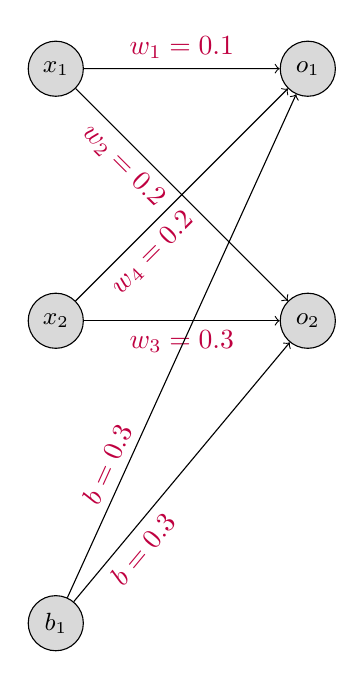
\begin{tikzpicture}[x=2cm,y=2cm] 
			\begin{scope}[scale=1.6]
			
			\tikzstyle{mycircle}=[circle,
			draw=black,
			fill=gray,
			fill opacity = 0.3,
			text opacity=1,
			inner sep=0pt,
			minimum size=7mm,
			font=\small
			]
			\tikzstyle{myline}=[-]
			\tikzstyle{myarrow}=[->]
			
			\coordinate (px1) at (-1, 1);
			\coordinate (px2) at (-1, 0);
			\coordinate (pb1) at (-1, -1.2);
			
			\coordinate (po1) at (0, 1);
			\coordinate (po2) at (0, 0);
			
			
			\node[mycircle] (x1) at (px1) {$x_1$};	
			\node[mycircle] (x2) at (px2) {$x_2$};	
			\node[mycircle] (b1) at (pb1) {$b_1$};	
			
			\node[mycircle] (o1) at (po1) {$o_1$};	
			\node[mycircle] (o2) at (po2) {$o_2$};	
			
			\draw[myarrow] (x1) -- node[purple, auto] {$w_1=0.1$} (o1);			
			\draw[myarrow] (x1) -- node[purple, sloped, anchor=x2, below left] {$w_2=0.2$} (o2);
			
			\draw[myarrow] (x2) -- node[purple, below] {$w_3=0.3$} (o2);			
			\draw[myarrow] (x2) -- node[purple, sloped, anchor=x2, below left] {$w_4=0.2$} (o1);
			
			
			\draw[myarrow] (b1) -- node[purple, sloped, above, near start] {$b=0.3$} (o1);
			\draw[myarrow] (b1) -- node[purple, sloped, below, near start] {$b=0.3$} (o2);
			
			\end{scope}
			\end{tikzpicture}
		\end{figure}
		\captionof{figure}{Multi-Layer Perceptron}
		\label{fig:Sheet5Ex1}
	\end{minipage}
	\hfill
	\begin{minipage}[b]{0.49\textwidth}
		\centering
		\begin{tabular}{ |c | c | c | c | c |}
			\hline
			$n$ & $x_1$ & $x_2$ & $p_1$ & $p_2$\\ \hline
			$1$ & $0.1$ & $0.4$ & $0.1$ & $0.9$\\ \hline
			$2$ & $0.8$ & $0.2$ & $0.95$ & $0.05$\\ \hline
			$3$ & $0.6$ & $0.5$ & $0.4$ & $0.6$\\ \hline
			$4$ & $0.3$ & $0.9$ & $0.75$ & $0.25$\\ \hline
			$5$ & $0.3$ & $0.5$ & $0.9$ & $0.1$\\ \hline
		\end{tabular}
		\captionof{table}{Training batch}
	\end{minipage}
\end{minipage}

\begin{algorithm}[H] 
	\caption{Generative Adversarial Networks (GAN)}%\label{alg:GAN}
	\begin{tabbing}
		\textbf{Output:} \= \kill
		\textbf{Input:} \> a discriminator function $D$,\\
		\> a generator function $G$,\\
		\> noise samples $Z$,\\
		\> true samples $X$ (with an underlying data generation distribution $\IP_{\text{data}}[X]$),\\
		\> desired size of mini-batches $m$,\\
		\> a number $k$ of improvement iterations for the discriminator,\\
		\> stopping criterion $T_{\text{condition}}$\\
		\textbf{Output:} \> a generator $G$ that is able to fool the trained discriminator $D$
	\end{tabbing}
	\begin{algorithmic}[1]
		\While {not $T_{\text{condition}}(f, \theta)$}
		\For {$k$ steps}
		\State Sample a minibatch of noise samples $\{z^{(1)}, \dots, z^{(m)}\}$
		\State Sample a minibatch of true samples $\{x^{(1)}, \dots, x^{(m)}\}$
		\State Perform stochastic gradient ascend for the discriminator:
		\[ \nabla_{\theta^{(d)}}\frac{1}{m}\sum\limits_{i=1}^{m}\Big( \log\big( d(x^{(i)};\theta^{(d)}) \big) + \log\big(1-d\big(g(z^{(i)};\theta^{(g)}),\theta^{(d)}\big)\big) \Big) \]
		\EndFor
		\State Sample a minibatch of noise samples $\{z^{(1)}, \dots, z^{(m)}\}$
		\State Perform stochastic gradient descending for the generator:
		\[ \nabla_{\theta^{(g)}}\frac{1}{m}\sum\limits_{i=1}^{m}\Big(  \log\big(1-d\big(g(z^{(i)};\theta^{(g)}),\theta^{(d)}\big)\big) \Big) \]
		\EndWhile
	\end{algorithmic}	
\end{algorithm}

%%%% ----------------------- %%%%
%%%% ------Bibliography----- %%%%
%%%% ----------------------- %%%%
\newpage
\printbibliography

\end{document}
